\documentclass[
  paper=a4,
  % version=3.25,
  pagesize=pdftex,
  twoside=false,
  toc=listof,
  BCOR=0pt,
  DIV=15,
  indent,
]{scrartcl}
\usepackage{ctex}
\usepackage{tcolorbox}
\usepackage{tkz-euclide}
\usetkzobj{all}
\usepackage{tikz}
\usepackage{pgfornament,amsmath}
\usetikzlibrary{shapes.symbols}
\usetikzlibrary{math, calc}
\usepackage{pdfpages}
\usepackage{tikz-network}
\usepackage{animate}
\usepackage{tikz-euclide-documentation}
\usepackage{pdfpages}


\newcommand{\MS}{Martin Scheidt}

\hypersetup{
  pdftitle={tikz/networkmanual},
  pdfsubject={A tikz toolbox for track schematics},
  pdfauthor={Latex Studio},
  pdfkeywords={latex, tikz, library, railway, track, layout}
}

\definecolor{myback}{RGB}{53,64,89}
\definecolor{mycolor}{RGB}{51,51,51}
\definecolor{Orange}{RGB}{102,51,0}
\definecolor{Green}{RGB}{0,102,51}
\definecolor{Blue}{RGB}{15,107,108}
\definecolor{Yellow}{RGB}{153,151,51}


\begin{document}

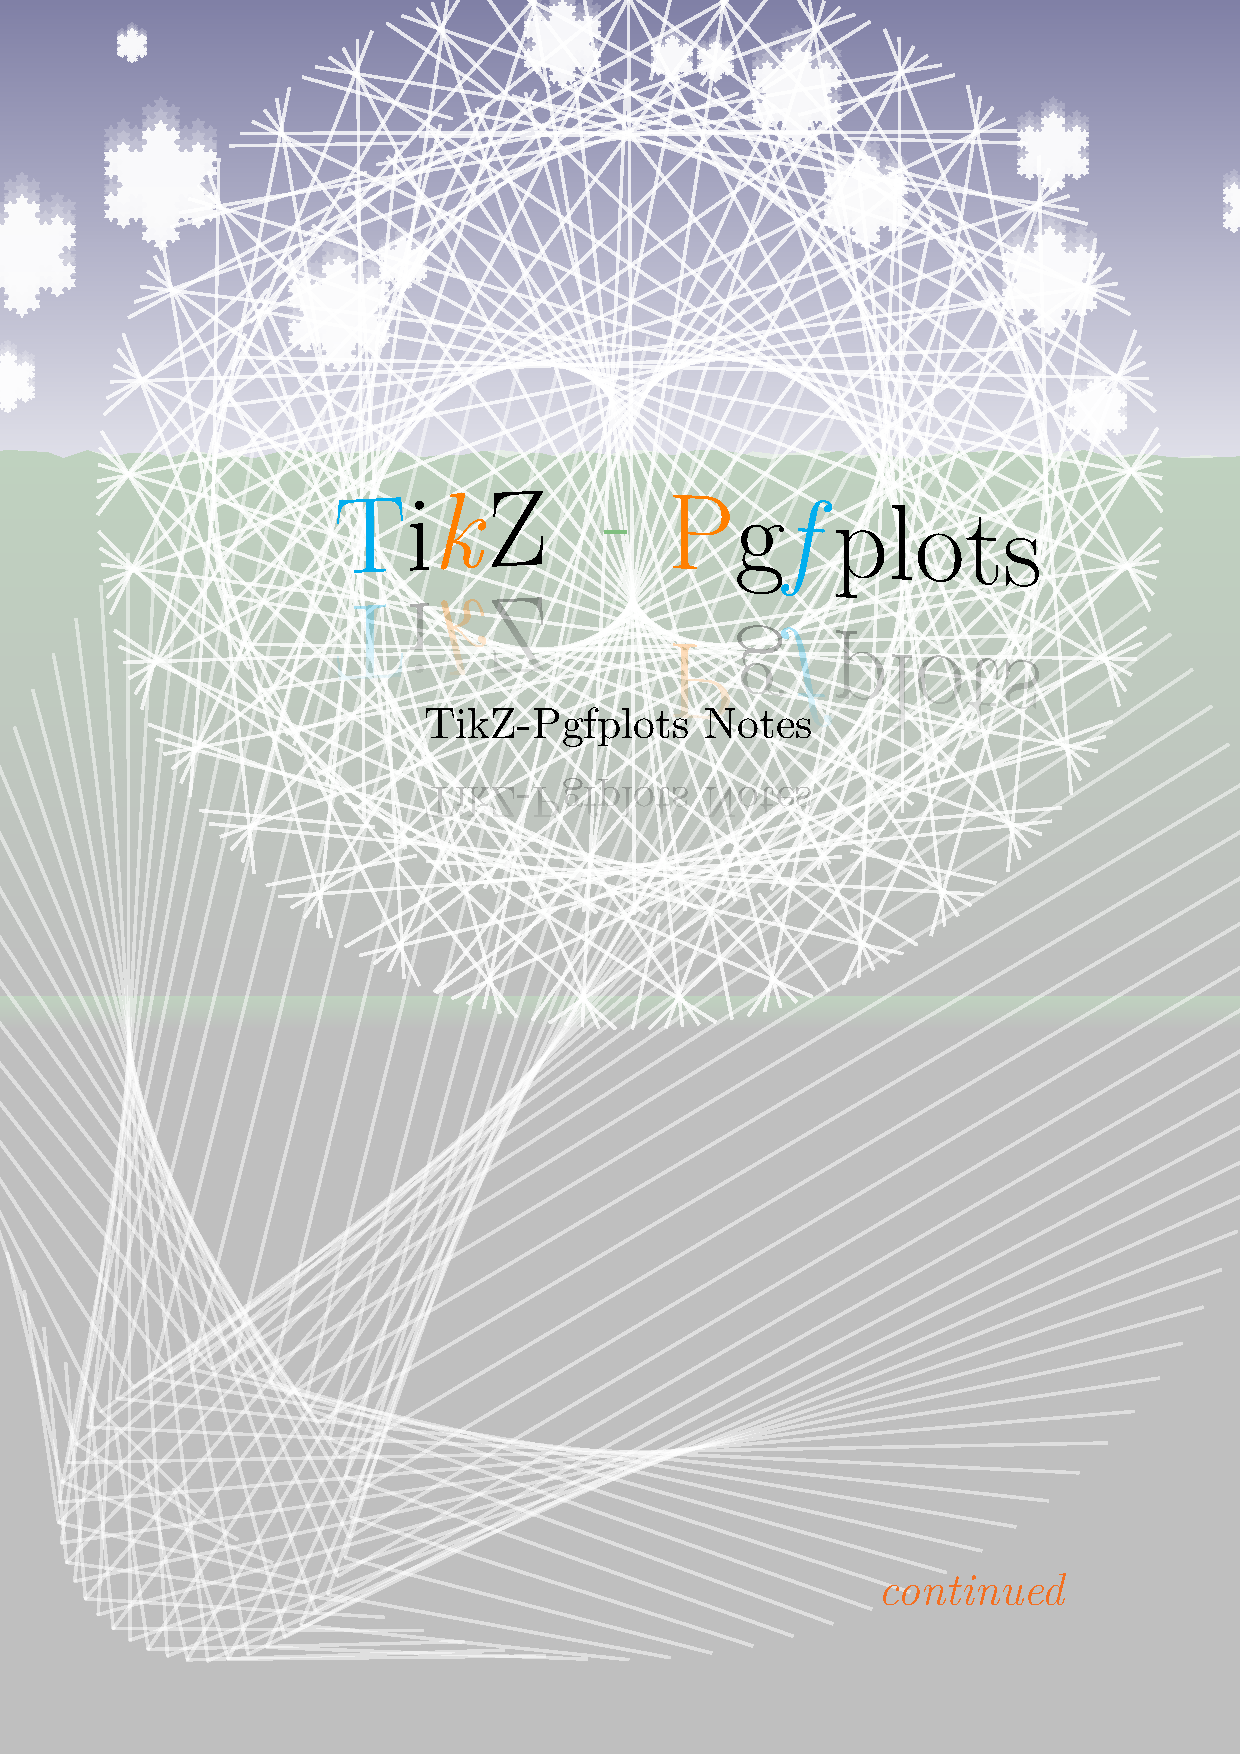
\includepdf[pages={1}]{Template_5fengmian.pdf}

\newpage

\title{\tikz\node[scale=1.2]{\color{gray}\Huge\sffamily \{\textcolor{black}{Ti\textcolor{orange}{\emph{k}}Z}-\textcolor{blue}{Pgfplotsapplication}\}};}
\subtitle{T\emph{k}Z \textcolor{orange}{\&} euclide  \textcolor{blue}{绘图应用}}
\author{\vhListAllAuthorsLong}
\date{Version 实用(进阶)篇}

\maketitle
\thispagestyle{empty}
\begin{multicols}{2}
  \tableofcontents
\end{multicols}
\vspace{1.5cm}
\begin{multicols}{2}
\centerline{
  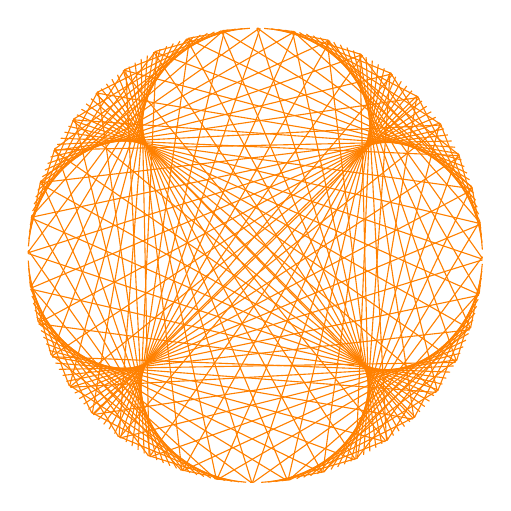
\begin{tikzpicture}[scale=0.8]
    \foreach \i in {0,0.01,...,2}
    \draw[draw=orange,rotate=-124]($(0,0) !1! \i*180:(3,2)$)--($(0,0) !1! \i*900:(3,2)$);
    \end{tikzpicture}
}

  \centerline{
    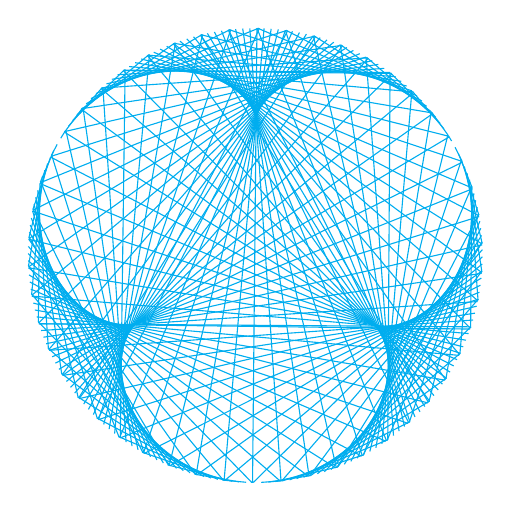
\begin{tikzpicture}[scale=0.8]
     \foreach \i in {0,0.01,...,2}
 \draw[draw=cyan,rotate=-124]($(0,0) !1! \i*180:(3,2)$)--($(0,0) !1! \i*720:(3,2)$);
    \end{tikzpicture}
  }
  \end{multicols}
  \vfill

 \quad \textcolor{red}{\Large $\star\star\star\star\star\star\star\star\star\star\star\star\star\star\star\star\star\star\star\star$ }~\textcolor{blue}{Yongxue Liu}~\textcolor{red}{\Large $\star\star\star\star\star\star\star\star\star\star\star\star\star\star\star\star\star\star\star\star$ }
\cleardoublepage

\begin{center}
{\Large\bfseries 前言}
\end{center}

\qquad 最近整理了一份~\LaTeX{} 绘图笔记,内容主要侧重于绘制中学学习教材上用到的大部分图,对于~\LaTeX{} 绘图的入门,初学者可以进入~\LaTeX{} 工作室官网寻找一些 TikZ 的绘图入门,其中有~\href{https://www.latexstudio.net/index/details/index/mid/940.html}{\textcolor{orange}{TikZ 绘图入门基础}}、\href{https://www.latexstudio.net/index/details/index/mid/878.html} {\textcolor{blue}{TikZ 学习笔记}}、\href{https://www.latexstudio.net/index/details/index/mid/949.html} {\textcolor{cyan}{TikZ/PGF manual}} 以及~TikZ 绘图宏包的学习手册。相关的资源可以关注公众号动态,以及工作室官方网站。

\begin{multicols}{2}
\centerline{
\includegraphics[scale=0.15]{fig2}}
\centerline{
\includegraphics[scale=0.1]{fig1}}
\end{multicols}

{\centering
\begin{tikzpicture}
  \begin{scope}[color=cyan]

  \node[minimum size=15cm](current page1){};
  \node[scale=0.5,anchor=north west] at (current page1.north west)
  {\pgfornament[width=7cm]{35}};
  \node[scale=0.5,anchor=west,rotate=45] at (current page1.west)
  {\pgfornament[width=7cm]{35}};
  \node[scale=0.5,anchor=north east] at (current page1.north east)
  {\pgfornament[width=7cm]{36}};
  \node[scale=0.5,anchor=east,rotate=-45] at (current page1.east)
  {\pgfornament[width=7cm]{36}};
  \node[scale=0.5,anchor=south west] at (current page1.south west)
  {\pgfornament[width=7cm,symmetry=h]{35}};
  \node[scale=0.5,anchor=south,rotate=45] at (current page1.south)
  {\pgfornament[width=7cm,symmetry=h]{35}};
  \node[scale=0.5,anchor=south east] at (current page1.south east)
  {\pgfornament[width=7cm,symmetry=h]{36}};
  \node[scale=0.5,anchor=south,rotate=-45] at (current page1.south)
  {\pgfornament[width=7cm,symmetry=h]{36}};
  \node[scale=20,green!45!black,cloud,cloud puffs=14,draw=blue,fill=pink]at(current page1.center){\scalebox{0.1}{~~~~~~~~}};
  \end{scope}

  \node[scale=1.45]at (0,0.7){
  \begin{tikzpicture}
 \foreach \i in {0,0.01,...,2}
     \draw[draw=white,rotate=-95,thick]($(0,0) !1! \i*180:(3,2)$)--($(1,0) !1! \i*360:(2,2)$);
     \begin{scope}
     \node[scale=2,green!45!black,rotate=55]at(-2.3,1.2){2};
     \node[scale=2,green!45!black,rotate=45]at(-2,1.5){0};
     \node[scale=2,green!45!black,rotate=40]at(-1.7,1.8){2};
     \node[scale=2,green!45!black,rotate=25]at(-1.3,2){0};
     \node[scale=2,green!45!black,rotate=-55]at(2.3,1.2){1};
     \node[scale=2,green!45!black,rotate=-45]at(2,1.5){2};
     \node[scale=2,green!45!black,rotate=-40]at(1.7,1.8){0};
     \node[scale=2,green!45!black,rotate=-25]at(1.3,2){2};
     \node[scale=2,green!45!black,rotate=0]at(0,4){Happy};
     \node[scale=1.5,green!45!black,rotate=0]at(0,2.8){New Year};
  \end{scope}
         \end{tikzpicture}};

  \end{tikzpicture}
}
\vspace{-1cm}
\textcolor{orange}{\dotfill}~\textit{全世界在等我飞更高~~你却心疼我受伤翅膀}
\thispagestyle{empty}
\clearpage
\thispagestyle{empty}
\begin{center}
{\Large\bfseries 分享}
\end{center}

\qquad 在学习~TikZ 绘图过程中,偶尔看见别人用~Blender 结合 Python 绘制心线图的动画视频,于是常识了用~\LaTeX 中 TikZ 宏包去实现,最后绘制出来了,这里进行代码分享!

首先是心线图的绘制:

%\noindent
%\textcolor{orange}{\dotfill}\\
\vspace{3pt}
\begin{minipage}[c]{0.51\textwidth}
  \centering
  \begin{lstlisting}[gobble=8]
        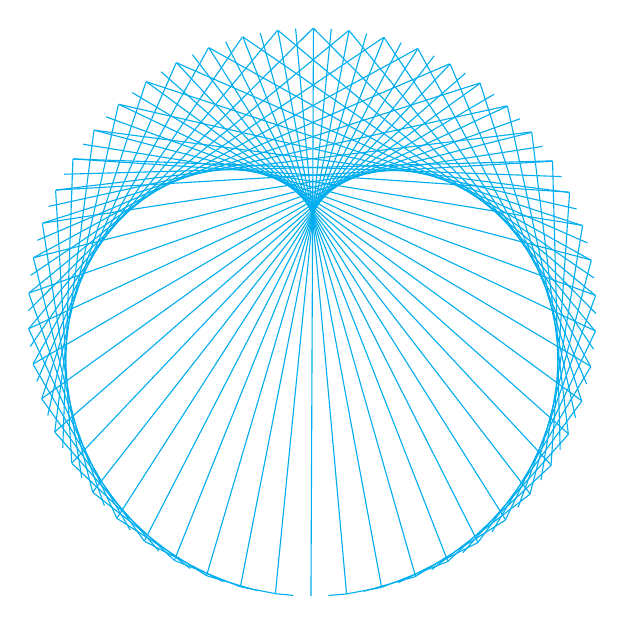
\begin{tikzpicture}
         \foreach \i in {0,0.02,...,2} % foreach 循环语句
           \draw
                [
                 draw=cyan,  % 绘制线条颜色
                 rotate=-124 % 旋转角度
                ]
                ($(0,0) !1! \i*180:
                (3,2)$)--($(0,0) !1! \i*360:(3,2)$);
                % 在圆上标记100个等分点,依次从0标记到99,每个点连接标记是它2倍
                %的点,最后形成心线!
        \end{tikzpicture}
  \end{lstlisting}
  \vspace{2pt}
\end{minipage}
\hfil
\begin{minipage}[c]{0.45\textwidth}
  \centering
  \vspace{3pt}
  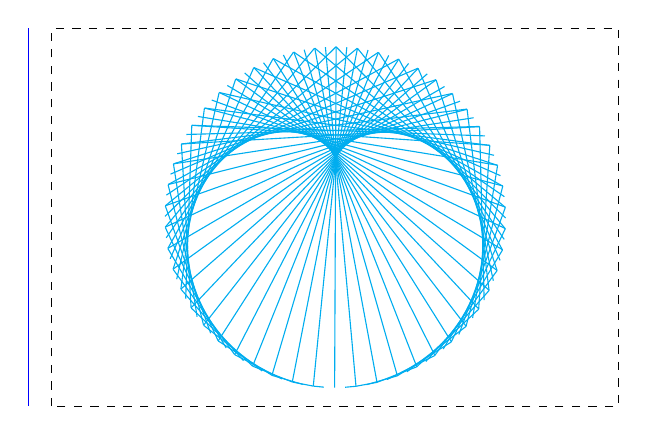
\begin{tikzpicture}[scale=0.6]
  \draw[blue](-6.5,-4)--(-6.5,4);
  \draw[dashed](-6,-4) rectangle (6,4);
  \foreach \i in {0,0.02,...,2}
  \draw[draw=cyan,rotate=-124]($(0,0) !1! \i*180:(3,2)$)--($(0,0) !1! \i*360:(3,2)$);
\end{tikzpicture}
\vspace{2pt}
\end{minipage}
%\noindent
%\textcolor{orange}{\rule{\textwidth}{0.6pt}}


类似地,我们连接的点变成3倍、4倍甚至n倍,以及小数点倍会是怎样的感觉呢,下面来看看:

\vspace{3pt}
\begin{minipage}[c]{0.51\textwidth}
  \centering
  \begin{lstlisting}[gobble=8]
        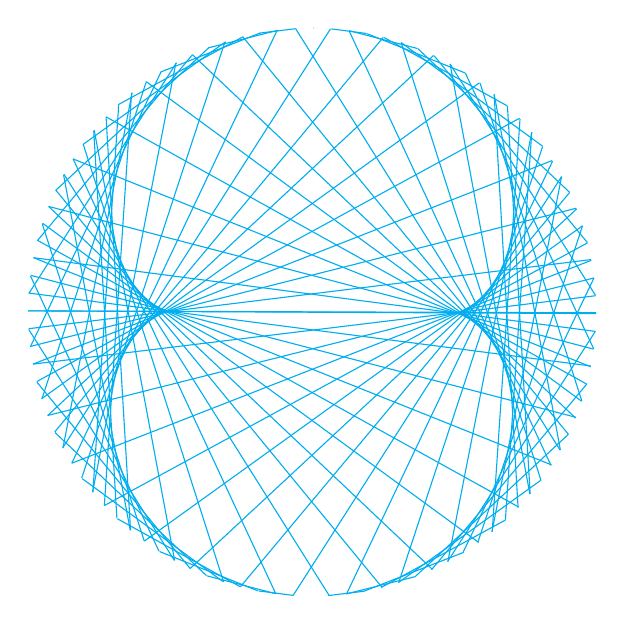
\begin{tikzpicture}
         \foreach \i in {0,0.02,...,2} % foreach 循环语句
           \draw
                [
                 draw=cyan,  % 绘制线条颜色
                 rotate=-124 % 旋转角度
                ]
                ($(0,0) !1! \i*180:(3,2)$)--($(0,0) !1! \i*540:(3,2)$);
                % 在圆上标记100个等分点,依次从0标记到99,每个点连接标记是它3倍
                %的点,最后形成心线!
        \end{tikzpicture}
  \end{lstlisting}
  \vspace{2pt}
\end{minipage}
\hfil
\begin{minipage}[c]{0.45\textwidth}
  \centering
  \vspace{3pt}
  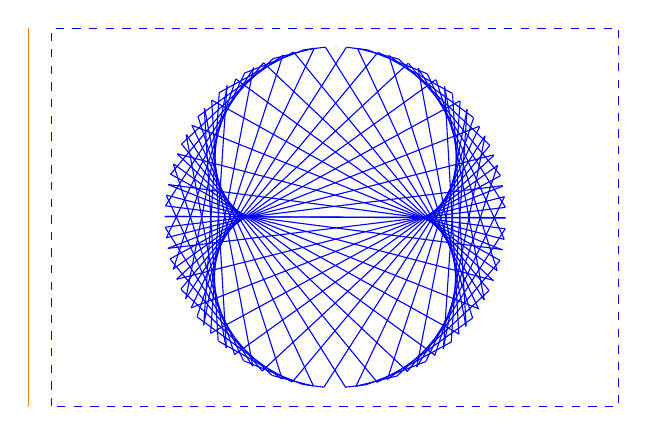
\begin{tikzpicture}[scale=0.6]
  \draw[orange](-6.5,-4)--(-6.5,4);
  \draw[draw=blue,dashed](-6,-4) rectangle (6,4);
  \foreach \i in {0,0.02,...,2}
  \draw[draw=blue,rotate=-124]($(0,0) !1! \i*180:(3,2)$)--($(0,0) !1! \i*540:(3,2)$);
\end{tikzpicture}
\vspace{2pt}
\end{minipage}

连接点数是其标记点数~4 倍的时候是这样的,图像如下:

\vspace{3pt}
\begin{minipage}[c]{0.51\textwidth}
  \centering
  \begin{lstlisting}[gobble=8]
        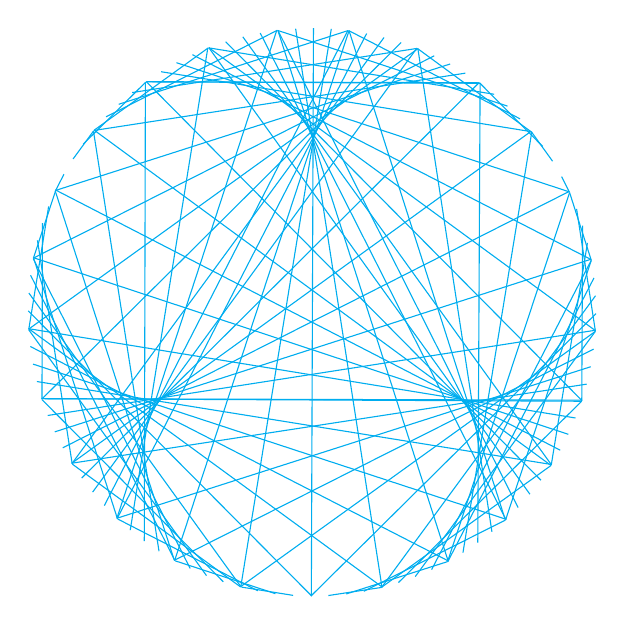
\begin{tikzpicture}
         \foreach \i in {0,0.02,...,2} % foreach 循环语句
           \draw
                [
                 draw=cyan,  % 绘制线条颜色
                 rotate=-124 % 旋转角度
                ]
                ($(0,0) !1! \i*180:(3,2)$)--($(0,0) !1! \i*720:(3,2)$);
                % 在圆上标记100个等分点,依次从0标记到99,每个点连接标记是它3倍
                %的点,最后形成心线!
        \end{tikzpicture}
  \end{lstlisting}
  \vspace{2pt}
\end{minipage}
\hfil
\begin{minipage}[c]{0.45\textwidth}
  \centering
  \vspace{3pt}
  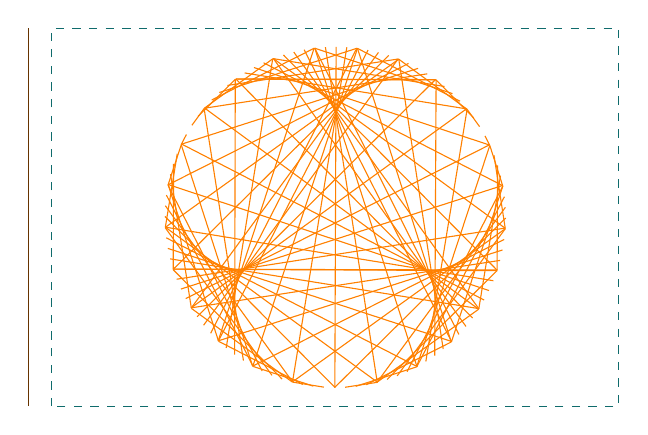
\begin{tikzpicture}[scale=0.6]
  \draw[Orange](-6.5,-4)--(-6.5,4);
  \draw[draw=Blue,dashed](-6,-4) rectangle (6,4);
  \foreach \i in {0,0.02,...,2}
  \draw[draw=orange,rotate=-124]($(0,0) !1! \i*180:(3,2)$)--($(0,0) !1! \i*720:(3,2)$);
\end{tikzpicture}
\vspace{2pt}
\end{minipage}

下列代码运行生成多页PDF格式文档,运用宏包~animate 制作动画:


\begin{lstlisting}[gobble=8]
        \documentclass{ctexart}
        \usepackage{ctex}
        \usepackage{amsmath}
        \usepackage{tikz}
        \usetikzlibrary{calc}\tikzset{>=latex}
        \usepackage{pgfplots}
        \usepackage[active,tightpage]{preview}
        \PreviewEnvironment{tikzpicture}
        \setlength\PreviewBorder{0pt}
        \definecolor{myback}{RGB}{53,64,89}
        \definecolor{mycolor}{RGB}{51,51,51}
        \definecolor{Orange}{RGB}{102,51,0}
        \definecolor{Green}{RGB}{0,102,51}
        \definecolor{Blue}{RGB}{15,107,108}
        \definecolor{Yellow}{RGB}{153,151,51}
        \begin{document}
                  \foreach \N in {0.1,0.0995,...,0}{
                          \begin{tikzpicture}
                            \draw[fill=myback](-6,-4) rectangle (6,5);
                            \draw[fill=myback](-6,-4) rectangle (6,4);
                                \foreach \i in {0,\N,...,2}
                            \draw[draw=orange!60!yellow,rotate=-124]($(0,0) !1! \i*180:(3,2)$)--($(0,0) !1! \i*400:(2,2)$);
                          \end{tikzpicture}}
        \end{document}
\end{lstlisting}
\thispagestyle{empty}
\vspace{3pt}
\begin{minipage}[c]{0.51\textwidth}
  \centering
  \begin{lstlisting}[gobble=8]
        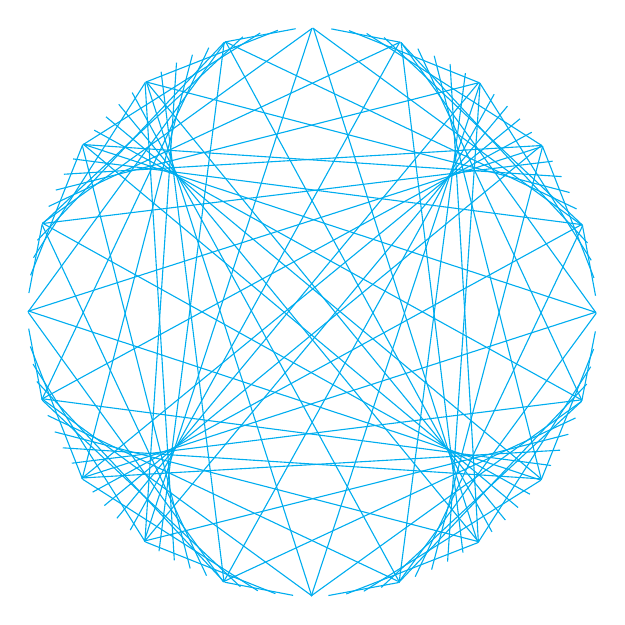
\begin{tikzpicture}
         \foreach \i in {0,0.02,...,2} % foreach 循环语句
           \draw
                [
                 draw=cyan,  % 绘制线条颜色
                 rotate=-124 % 旋转角度
                ]
                ($(0,0) !1! \i*180:(3,2)$)--($(0,0) !1! \i*900:(3,2)$);
                % 在圆上标记100个等分点,依次从0标记到99,每个点连接标记是它3倍
                %的点,最后形成心线!
        \end{tikzpicture}
  \end{lstlisting}
  \vspace{2pt}
\end{minipage}
\hfil
\begin{minipage}[c]{0.45\textwidth}
  \centering
  \vspace{3pt}
  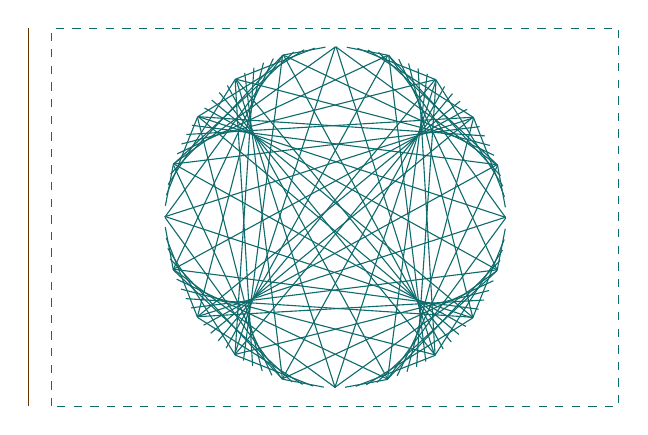
\begin{tikzpicture}[scale=0.6]
  \draw[Orange](-6.5,-4)--(-6.5,4);
  \draw[draw=Blue,dashed](-6,-4) rectangle (6,4);
  \foreach \i in {0,0.02,...,2}
  \draw[draw=Blue,rotate=-124]($(0,0) !1! \i*180:(3,2)$)--($(0,0) !1! \i*900:(3,2)$);
\end{tikzpicture}
\vspace{2pt}
\end{minipage}


\vspace{3pt}
\begin{minipage}[c]{0.51\textwidth}
  \centering
  \begin{lstlisting}[gobble=8]
        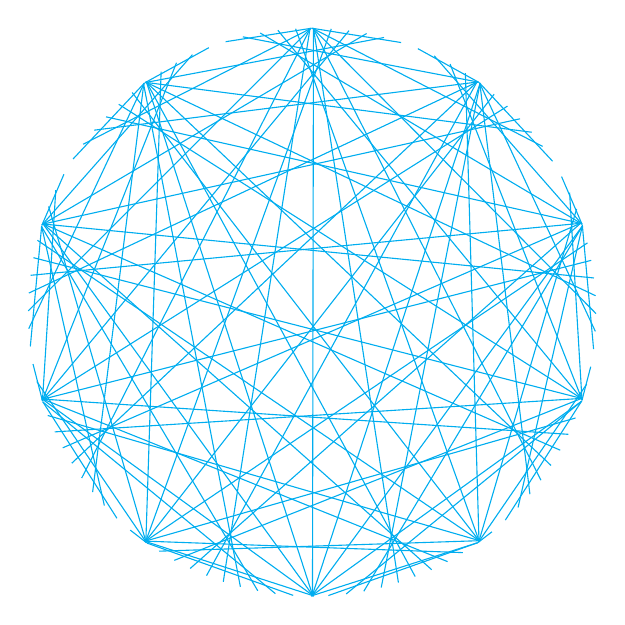
\begin{tikzpicture}
         \foreach \i in {0,0.02,...,2} % foreach 循环语句
           \draw
                [
                 draw=cyan,  % 绘制线条颜色
                 rotate=-124 % 旋转角度
                ]
                ($(0,0) !1! \i*180:(3,2)$)--($(0,0) !1! \i*1800:(3,2)$);
                % 在圆上标记100个等分点,依次从0标记到99,每个点连接标记是它3倍
                %的点,最后形成心线!
        \end{tikzpicture}
  \end{lstlisting}
  \vspace{2pt}
\end{minipage}
\hfil
\begin{minipage}[c]{0.45\textwidth}
  \centering
  \vspace{3pt}
  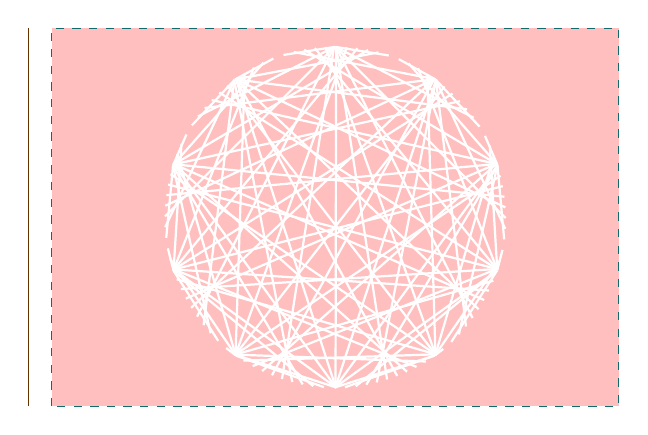
\begin{tikzpicture}[scale=0.6]
  \draw[Orange](-6.5,-4)--(-6.5,4);
  \draw[draw=Blue,dashed,fill=pink](-6,-4) rectangle (6,4);
  \foreach \i in {0,0.02,...,2}
  \draw[draw=white,rotate=-124,thick]($(0,0) !1! \i*180:(3,2)$)--($(0,0) !1! \i*1800:(3,2)$);
\end{tikzpicture}
\vspace{2pt}
\end{minipage}

\vspace{-3pt}
\begin{minipage}[c]{0.51\textwidth}
  \centering
  \begin{lstlisting}[gobble=8]
        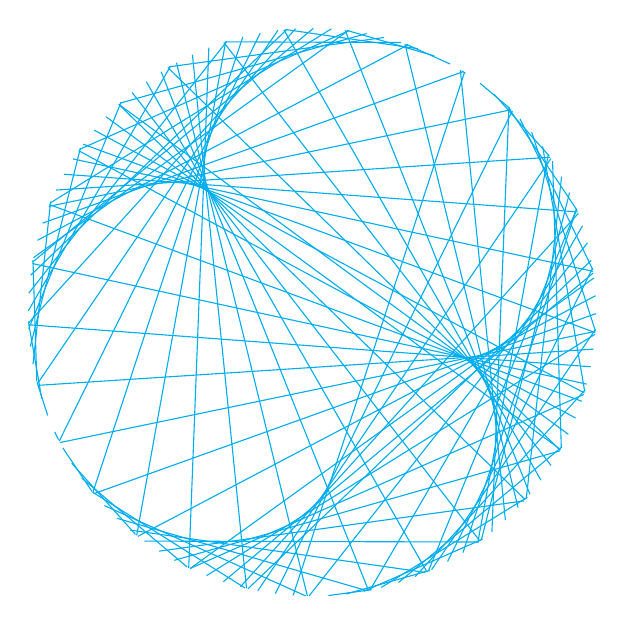
\begin{tikzpicture}
         \foreach \i in {0,0.02,...,2} % foreach 循环语句
           \draw
                [
                 draw=cyan,  % 绘制线条颜色
                 rotate=-124 % 旋转角度
                ]
                ($(0,0) !1! \i*180:(3,2)$)--($(0,0) !1! \i*620:(3,2)$);
                % 在圆上标记100个等分点,依次从0标记到99,每个点连接标记是它3倍
                %的点,最后形成心线!
        \end{tikzpicture}
  \end{lstlisting}
  \vspace{2pt}
\end{minipage}
\hfil
\begin{minipage}[c]{0.45\textwidth}
  \centering
  \vspace{3pt}
  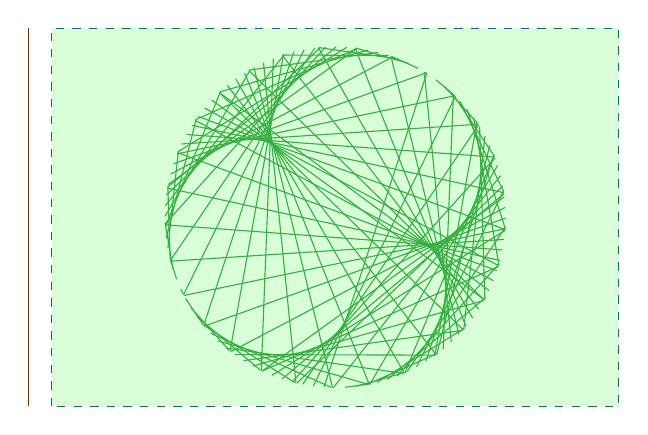
\begin{tikzpicture}[scale=0.6]
  \draw[Orange](-6.5,-4)--(-6.5,4);
  \draw[draw=Blue,dashed,fill=green!15!white](-6,-4) rectangle (6,4);
  \foreach \i in {0,0.02,...,2}
  \draw[draw=yellow!80!red!20!green,rotate=-124]($(0,0) !1! \i*180:(3,2)$)--($(0,0) !1! \i*620:(3,2)$);
\end{tikzpicture}
\vspace{2pt}
\end{minipage}


\vspace{3pt}
\begin{minipage}[c]{0.51\textwidth}
  \centering
  \begin{lstlisting}[gobble=8]
        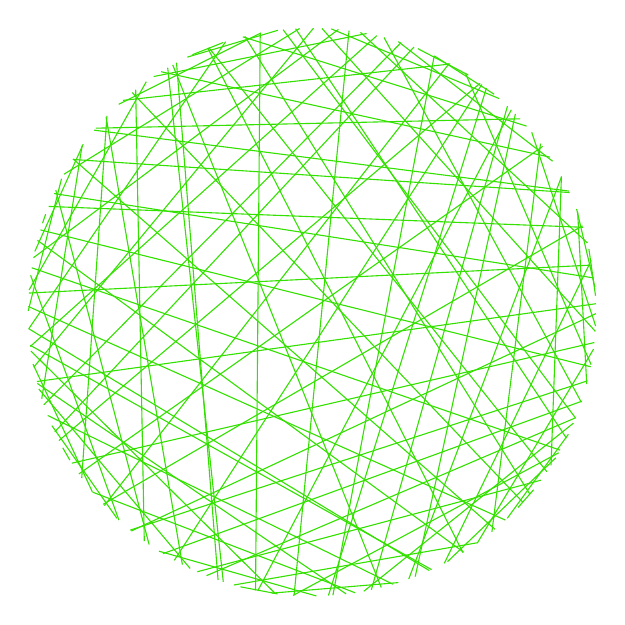
\begin{tikzpicture}
          \foreach \i in {0,0.02,...,2}
          \draw[
          draw=orange!80!red!20!green,
          rotate=-124
          ]($(0,0)
          !1! \i*180:(3,2)$)--($(0,0) !1!
          \i*7120:(3,2)$);
        \end{tikzpicture}
  \end{lstlisting}
  \vspace{2pt}
\end{minipage}
\hfil
\begin{minipage}[c]{0.45\textwidth}
  \centering
  \vspace{3pt}
  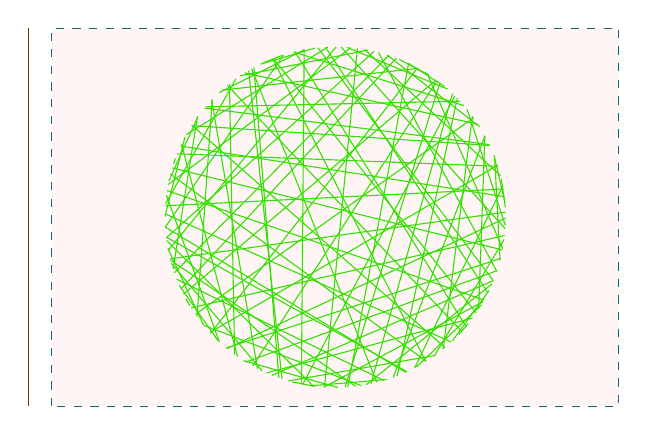
\begin{tikzpicture}[scale=0.6]
  \draw[Orange](-6.5,-4)--(-6.5,4);
  \draw[draw=Blue,dashed,fill=pink!15!white](-6,-4) rectangle (6,4);
  \foreach \i in {0,0.02,...,2}
  \draw[draw=orange!80!red!20!green,rotate=-124]($(0,0) !1! \i*180:(3,2)$)--($(0,0) !1! \i*7120:(3,2)$);
\end{tikzpicture}
\vspace{2pt}
\end{minipage}

\thispagestyle{empty}


\begin{tikzpicture}
    \node at (0,2) {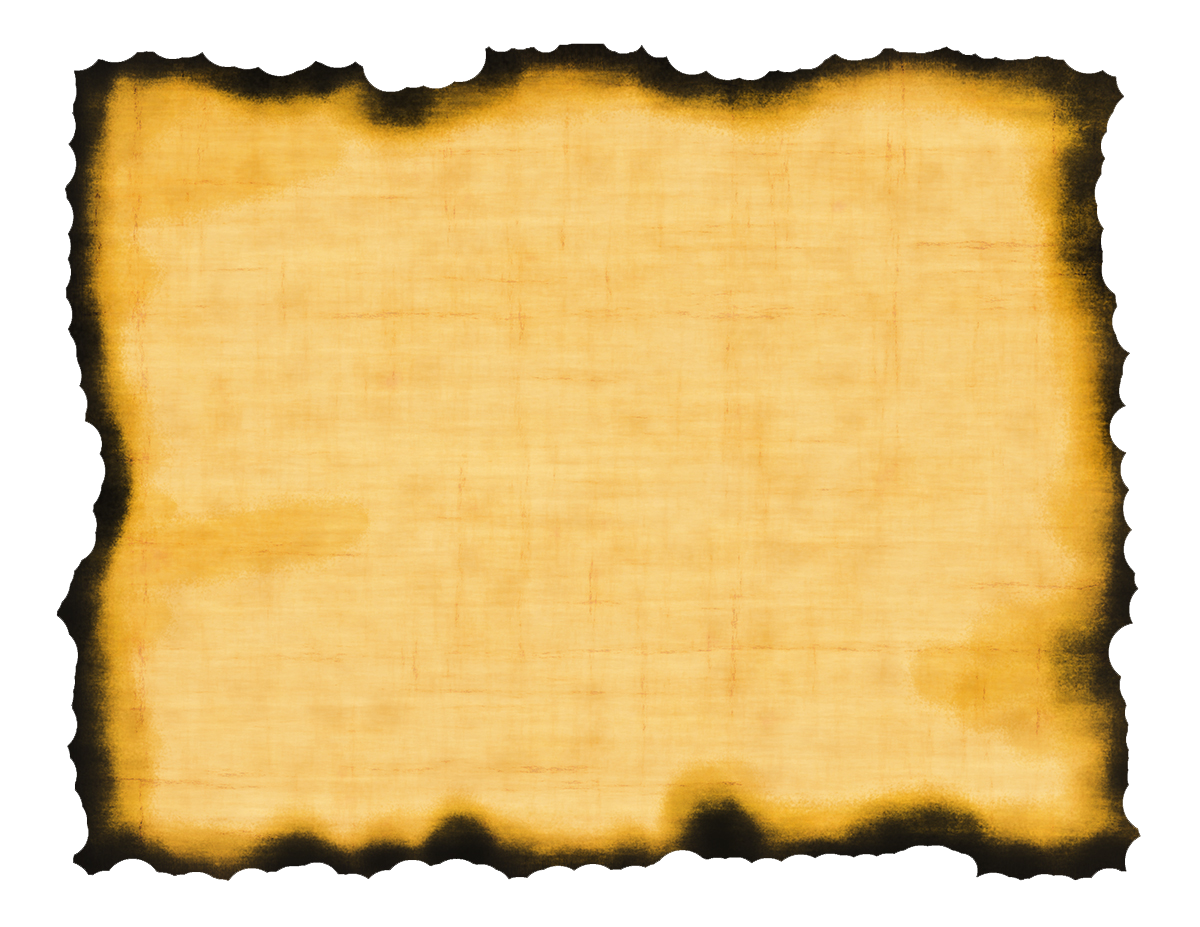
\includegraphics[width=480bp]{papiro.png}};
    \node at (0,3.5) [rectangle]{\parbox{350bp}{
      \begin{center}
        {\Huge\bfseries  内容简要}
        \end{center}
      {\Large\bfseries
        这部分我整理了在绘图学习中一些~Tikz 绘图的笔记,部分图是学习手册上的、部分是自己绘制的、也有自己搜集的其他人绘制的图,这些图主要的特点就是在生活工作尤其是教育教学,科研学术上用到,具体的内容包括:}
        {\bfseries
        \begin{enumerate}[label=\arabic*.,topsep=.5em]
            \setlength\parskip{.1em}
            \setlength{\baselineskip}{10pt}
            \item TikZ/PGFplots 曲线图绘制
            \item TikZ/PGFplots 柱状图/立体图绘制
            \item TikZ/PGFplots + Animate 动图绘制案例收集
            \item Pgfplots 学术绘图
            \end{enumerate}}

            \vfill
                      图片来源:https://codeload.github.com/livro-aberto/fracoes\_livro\_piloto/zip/master
                      }

                 };

                \end{tikzpicture}

\vfill
\dotfill~~\href{http://www.latexstudio.net.}{\textcolor{cyan}{LaTeX 工作室}}

\clearpage
 \section{TikZ/PGFplots 曲线的绘制}
 \thispagestyle{empty}
 \subsection{一般函数曲线的绘制}

 曲线的绘制,我认为能够根据函数表达式,在确定好自变量区间,然后选择适当的坐标轴比例,就可以绘制是最方便的,毕竟不需要描点连线等繁琐的步骤,至于对绘图最后装饰则需要根据你自己的需要即可,根据函数表达式绘图,我们给出一些案例:

 \textbf{多项式函数的绘制}

 \begin{lstlisting}[gobble=8]
          %  \definecolor{myback}{RGB}{53,64,89}
          %  \definecolor{mycolor}{RGB}{51,51,51}
          %  \definecolor{Orange}{RGB}{102,51,0}
          %  \definecolor{Green}{RGB}{0,102,51}
          %  \definecolor{Blue}{RGB}{15,107,108}
          %  \definecolor{Yellow}{RGB}{153,151,51}
        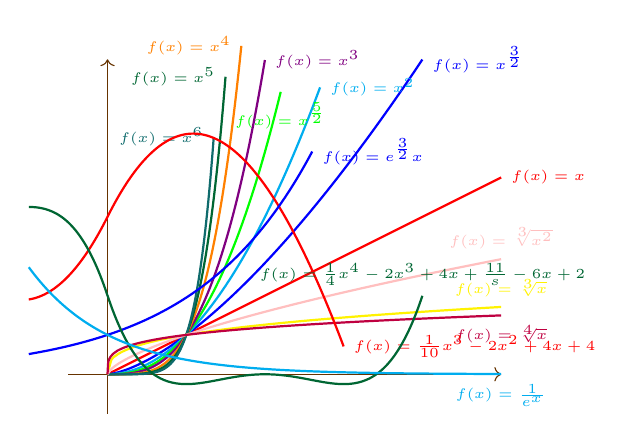
\begin{tikzpicture}[yscale=0.5]
          \draw[->,Orange](-0.5,0)--(5,0);
          \draw[->,Orange](0,-1)--(0,8);
          \draw[color=red, thick, domain=0:5,smooth,samples=100] plot ({\x},{\x}) node[right] {\tiny\(f(x)=x\)};
          \draw[color=blue,thick,domain=0:4,smooth,samples=100] plot ({\x},{\x^(3/2)}) node[right] {\tiny\(f(x)=x^\frac{3}{2}\)};
          \draw[color=cyan, thick, domain=0:2.7,smooth, samples=100] plot ({\x},{\x^(2)}) node[right] {\tiny\(f(x)=x^2\)};
          \draw[color=green,thick,domain=0:2.2,smooth,samples=100]plot({\x},{\x^(5/2)}) node[below] {\tiny\(f(x)=x^\frac{5}{2}\)};
          \draw[color=violet, thick, domain=0:2,smooth, samples=100] plot ({\x},{\x^(3)}) node[right] {\tiny\(f(x)=x^3\)};
          \draw[color=orange, thick, domain=0:1.7,smooth, samples=100] plot ({\x},{\x^(4)}) node[left] {\tiny\(f(x)=x^4\)};
          \draw[color=Green, thick, domain=0:1.5,smooth, samples=100] plot ({\x},{\x^(5)}) node[left] {\tiny\(f(x)=x^5\)};
          \draw[color=Blue, thick, domain=0:1.35,smooth, samples=100] plot ({\x},{\x^(6)}) node[left] {\tiny\(f(x)=x^6\)};
          \draw[color=yellow,thick,domain=0:5,smooth, samples=100] plot ({\x},{\x^(1/3)}) node[above] {\tiny\(f(x)=\sqrt[3]{x}\)};
          \draw[color=pink, thick,domain=0:5,smooth,samples=100] plot ({\x},{\x^(2/3)}) node[above] {\tiny\(f(x)=\sqrt[3]{x^2}\)};
          \draw[color=purple,thick,domain=0:5,smooth,samples=600] plot ({\x},{\x^(1/4)}) node[below] {\tiny\(f(x)=\sqrt[4]{x}\)};
          % 右边三个函数图像的绘制
          \draw[color=red, thick, domain=-1:3,smooth, samples=100] plot ({\x},{(1/10)*\x^(3)-2*\x^(2)+4*\x+4}) node[right] {\tiny\(f(x)=\frac{1}{10}x^3-2x^2+4x+4\)};
          \draw[color=blue, thick, domain=-1:2.6,smooth, samples=100] plot ({\x},{e^((2/3)*\x)}) node[right] {\tiny\(f(x)=e^\frac{3}{2}x\)};
          \draw[color=Green, thick, domain=-1:4,smooth, samples=100] plot ({\x},{(1/4)*\x^(4)-2*\x^(3)+(11/2)*\x^2-6*\x+2}) node[above] {\tiny\(f(x)=\frac{1}{4}x^4-2x^3+4x+\frac{11}{s}-6x+2\)};
          \draw[color=cyan,thick,domain=-1:5,smooth,samples=100] plot ({\x},{e^(-\x)}) node[below] {\tiny\(f(x)=\frac{1}{e^x}\)};
        \end{tikzpicture}
 \end{lstlisting}

 \vspace{3pt}
 \hfil\begin{minipage}[c]{0.51\textwidth}
  \begin{tikzpicture}[scale=0.6]
    \draw[draw=Blue,dashed,fill=cyan!15!white](-6,-4) rectangle (6,4);
    \node[scale=1] at (-0.5,0) {
      \begin{tikzpicture}[yscale=0.5]
        \draw[->,Orange](-0.5,0)--(5,0);
  \draw[->,Orange](0,-1)--(0,8);
  \draw[color=red, thick, domain=0:5,smooth, samples=100]
        plot ({\x},{\x}) node[right] {\tiny\(f(x)=x\)};
  \draw[color=blue, thick, domain=0:4,smooth, samples=100]
        plot ({\x},{\x^(3/2)}) node[right] {\tiny\(f(x)=x^\frac{3}{2}\)};
  \draw[color=cyan, thick, domain=0:2.7,smooth, samples=100]
        plot ({\x},{\x^(2)}) node[right] {\tiny\(f(x)=x^2\)};
  \draw[color=green, thick, domain=0:2.2,smooth, samples=100]
        plot ({\x},{\x^(5/2)}) node[below] {\tiny\(f(x)=x^\frac{5}{2}\)};
  \draw[color=violet, thick, domain=0:2,smooth, samples=100]
        plot ({\x},{\x^(3)}) node[right] {\tiny\(f(x)=x^3\)};
  \draw[color=orange, thick, domain=0:1.7,smooth, samples=100]
        plot ({\x},{\x^(4)}) node[left] {\tiny\(f(x)=x^4\)};
  \draw[color=Green, thick, domain=0:1.5,smooth, samples=100]
        plot ({\x},{\x^(5)}) node[left] {\tiny\(f(x)=x^5\)};
  \draw[color=Blue, thick, domain=0:1.35,smooth, samples=100]
        plot ({\x},{\x^(6)}) node[left] {\tiny\(f(x)=x^6\)};
  \draw[color=yellow, thick, domain=0:5,smooth, samples=100]
        plot ({\x},{\x^(1/3)}) node[above] {\tiny\(f(x)=\sqrt[3]{x}\)};
  \draw[color=pink, thick, domain=0:5,smooth, samples=100]
        plot ({\x},{\x^(2/3)}) node[above] {\tiny\(f(x)=\sqrt[3]{x^2}\)};
  \draw[color=purple!20!red, thick, domain=0:5,smooth, samples=600]
        plot ({\x},{\x^(1/4)}) node[below] {\tiny\(f(x)=\sqrt[4]{x}\)};
   \end{tikzpicture}
    };

  \end{tikzpicture}
  \vspace{2pt}
\end{minipage}
\quad
\begin{minipage}[c]{0.45\textwidth}
  \centering
  \vspace{3pt}
  \begin{tikzpicture}[scale=0.6]
 % \draw[Orange](-6.5,-4)--(-6.5,4);
  \draw[draw=Blue,dashed,fill=cyan!15!white](-6,-4) rectangle (6,4);
  \node[scale=1] at (0.5,0) {
    \begin{tikzpicture}[yscale=0.5]
      \draw[->,Orange](-0.5,0)--(5,0);
\draw[->,Orange](0,-1)--(0,8);
\draw[color=red, thick, domain=-1:3,smooth, samples=100]
      plot ({\x},{(1/10)*\x^(3)-2*\x^(2)+4*\x+4}) node[right] {\tiny\(f(x)=\frac{1}{10}x^3-2x^2+4x+4\)};
\draw[color=blue, thick, domain=-1:2.6,smooth, samples=100]
      plot ({\x},{e^((2/3)*\x)}) node[right] {\tiny\(f(x)=e^\frac{3}{2}x\)};
\draw[color=Green, thick, domain=-1:4,smooth, samples=100]
      plot ({\x},{(1/4)*\x^(4)-2*\x^(3)+(11/2)*\x^2-6*\x+2}) node[above] {\tiny\(f(x)=\frac{1}{4}x^4-2x^3+4x+\frac{11}{s}-6x+2\)};
 \draw[color=cyan, thick, domain=-1:5,smooth, samples=100]
      plot ({\x},{e^(-\x)}) node[below] {\tiny\(f(x)=\frac{1}{e^x}\)};
 \end{tikzpicture}
  };

\end{tikzpicture}
\vspace{2pt}
\end{minipage}

\textbf{三角函数图像的绘制}

三角函数基本绘图命令:

\begin{lstlisting}[gobble=8]
        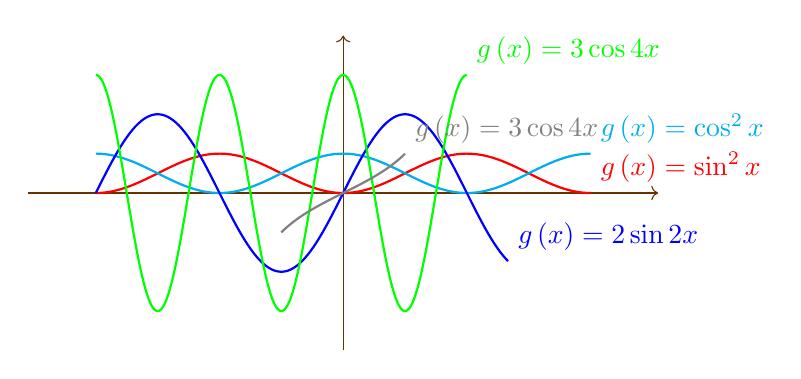
\begin{tikzpicture}[yscale=0.5]
        \draw[->,Orange](-4,0)--(4,0);
        \draw[->,Orange](0,-4)--(0,4);
        \draw[color=red, thick, domain=-pi:pi,smooth, samples=200] plot ({\x},{(sin(\x r))^2}) node[above right] {\(g\left(x\right)=\sin^2 x\)};
        \draw[color=cyan, thick, domain=-pi:pi,smooth, samples=200] plot ({\x},{(cos(\x r))^2}) node[above right] {\(g\left(x\right)=\cos^2 x\)};
        \draw[color=blue, thick, domain=-pi:(2/3)*pi,smooth, samples=200] plot ({\x},{(2*sin(2*\x r))}) node[above right] {\(g\left(x\right)=2\sin 2 x\)};
        \draw[color=green, thick, domain=-pi:(1/2)*pi,smooth, samples=200] plot ({\x},{(3*cos(4*\x r))}) node[above right] {\(g\left(x\right)=3\cos 4 x\)};
        \draw[color=gray, thick, domain=-(1/4)*pi:(1/4)*pi,smooth, samples=200] plot ({\x},{(tan(\x r))}) node[above right] {\(g\left(x\right)=3\cos 4 x\)};
        \end{tikzpicture}
\end{lstlisting}

\vspace{3pt}
\begin{minipage}[c]{0.51\textwidth}
  \centering
  \begin{lstlisting}[gobble=8]
        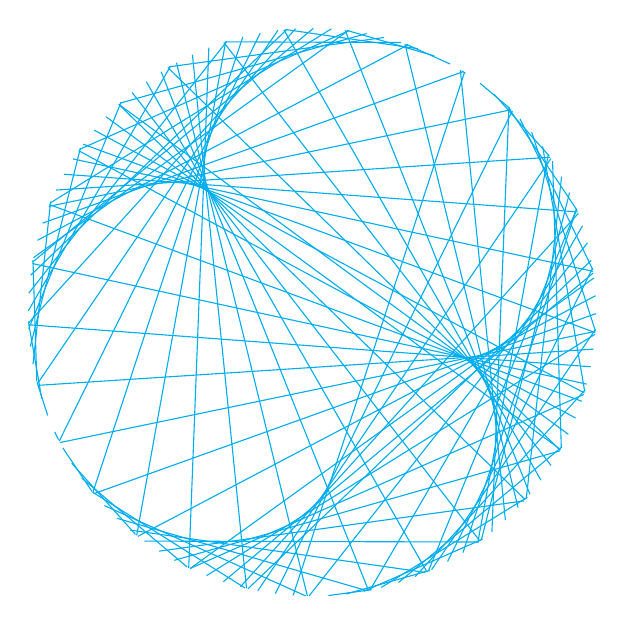
\begin{tikzpicture}
         \foreach \i in {0,0.02,...,2} % foreach 循环语句
           \draw
                [
                 draw=cyan,  % 绘制线条颜色
                 rotate=-124 % 旋转角度
                ]
                ($(0,0) !1! \i*180:(3,2)$)--($(0,0) !1! \i*620:(3,2)$);
                % 在圆上标记100个等分点,依次从0标记到99,每个点连接标记是它3倍
                %的点,最后形成心线!
        \end{tikzpicture}
  \end{lstlisting}
  \vspace{2pt}
\end{minipage}
\hfil
\begin{minipage}[c]{0.45\textwidth}
  \centering
  \vspace{3pt}
  \begin{tikzpicture}[scale=0.6]
     \draw[Orange,dashed](-6.5,-4)--(-6.5,4);
     \draw[draw=Blue,dashed,fill=cyan!15!white](-6,-4) rectangle (6,4);
     \node[scale=1] at (0,0) {
       \begin{tikzpicture}[yscale=0.5]
         \draw[->,Orange](-4,0)--(4,0);
   \draw[->,Orange](0,-4)--(0,4);
   \draw[color=red, thick, domain=-pi:pi,smooth, samples=200] plot ({\x},{(sin(\x r))^2}) node[above right] {\(g\left(x\right)=\sin^2 x\)};
   \draw[color=cyan, thick, domain=-pi:pi,smooth, samples=200] plot ({\x},{(cos(\x r))^2}) node[above right] {\(g\left(x\right)=\cos^2 x\)};
   \draw[color=blue, thick, domain=-pi:(2/3)*pi,smooth, samples=200] plot ({\x},{(2*sin(2*\x r))}) node[above right] {\(g\left(x\right)=2\sin 2 x\)};
   \draw[color=green, thick, domain=-pi:(1/2)*pi,smooth, samples=200] plot ({\x},{(3*cos(4*\x r))}) node[above right] {\(g\left(x\right)=3\cos 4 x\)};
  %  \draw[color=gray, thick, domain=-(1/4)*pi:(1/4)*pi,smooth, samples=200] plot ({\x},{(tan(\x r))}) node[above right] {\(g\left(x\right)=3\cos 4 x\)};
    \end{tikzpicture}
     };

   \end{tikzpicture}
\vspace{2pt}
\end{minipage}
\thispagestyle{empty}
\begin{center}
  \begin{tikzpicture}[scale=1]
    \draw[draw=Blue,dashed,fill=cyan!15!white](-6,-4) rectangle (6,4);
    \node[scale=1] at (0,0) {
      \begin{tikzpicture}[yscale=0.025]
        \draw[->,Orange](-6,0)--(6,0);
        \draw[->,Orange](0,-100)--(0,100);
   \draw[color=blue, thick, domain=-pi:pi,smooth, samples=200] plot ({\x},{(tan(\x r))})
   node[above right] {\(g\left(x\right)=\tan x\)};
   \draw[color=cyan, thick, domain=-pi:pi,smooth, samples=600] plot ({\x},{((1/8)*tan(20*\x r))})
   node[below right] {\(g\left(x\right)=\frac{1}{8}\tan 20x\)};

% \draw[color=gray, thick, domain=-1:1,smooth, samples=200,yscale=40] plot ({\x},{(rad(asin(\x)))}) node[above right] {\(g\left(x\right)=3\cos 4 x\)};
%  \draw[color=gray, thick, domain=-(1/4)*pi:(1/4)*pi,smooth, samples=200] plot ({\x},{(tan(\x r))}) node[above right] {\(g\left(x\right)=3\cos 4 x\)};
% \draw[color=gray, thick, domain=-(1/4)*pi:(1/4)*pi,smooth, samples=200] plot ({\x},{(tan(\x r))}) node[above right] {\(g\left(x\right)=3\cos 4 x\)};
   \end{tikzpicture}
    };
    \node[scale=1] at (5.5,3) {\begin{minipage}{0.4\textwidth}
      \begin{lstlisting}[gobble=8]
        \draw[color=cyan, thick, domain=-pi:pi,smooth,
         samples=600] plot ({\x},{((1/8)*tan(20*\x r))})
      node[below right] {\(g\left(x\right)=\frac{1}{8}\tan 20x\)};
      \end{lstlisting}
    \end{minipage}
    };

    \node[scale=1] at (-4,3) {\begin{minipage}{0.4\textwidth}
      \begin{lstlisting}[gobble=8]
        \draw[color=blue, thick, domain=-pi:pi,smooth,
         samples=200] plot ({\x},{(tan(\x r))})
        node[above right] {\(g\left(x\right)=\tan x\)};
      \end{lstlisting}
    \end{minipage}
    };
  \end{tikzpicture}
\end{center}


\begin{minipage}[c]{0.51\textwidth}
  \centering
  \begin{lstlisting}[gobble=8]
    \begin{tikzpicture}[yscale=0.5]
    \draw[color=red, thick, domain=-1:1,smooth, samples=200] plot ({\x},{(rad(sin(\x r)))}) node[above right] {\(g\left(x\right)=\text{arcsin}^2 x\)};
    \draw[color=cyan, thick, domain=-1:1,smooth, samples=200] plot ({\x},{rad(acos(\x r))}) node[above right] {\(g\left(x\right)=\text{arccos}^2 x\)};
    \draw[color=blue, thick, domain=-50:50,smooth, samples=200,xscale=0.1] plot ({\x},{rad(atan(\x r))}) node[above right] {\(g\left(x\right)=\text{arctan x}\)};
  \end{tikzpicture}
  \end{lstlisting}
  \vspace{2pt}
\end{minipage}
\hfil
\begin{minipage}[c]{0.45\textwidth}
  \centering
  \vspace{3pt}
  \begin{tikzpicture}[scale=0.6]
     \draw[Orange,dashed](-6.5,-4)--(-6.5,4);
     \draw[draw=Blue,dashed,fill=cyan!15!white](-6,-4) rectangle (6,4);
     \node[scale=1] at (0,0) {
       \begin{tikzpicture}[yscale=0.5]
         \draw[->,Orange](-4,0)--(4,0);
         \draw[dashed,green](-1,-4)--(-1,4);
         \draw[dashed,green](1,-4)--(1,4);
   \draw[->,Orange](0,-4)--(0,4);
   \draw[color=red, thick, domain=-1:1,smooth, samples=200] plot ({\x},{(rad(asin(\x)))}) node[above=0.2cm] {\(g\left(x\right)=\text{arcsin} x\)};
    \draw[color=cyan, thick, domain=-1:1,smooth, samples=200] plot ({\x},{(rad(acos(\x)))}) node[above right] {\(g\left(x\right)=\text{arccos}x\)};
    \draw[color=blue, thick, domain=-30:30,smooth, samples=600,xscale=0.1] plot ({\x},{rad(atan(\x))}) node[above right] {\(g\left(x\right)=\text{arctan x}\)};
    \end{tikzpicture}
     };

   \end{tikzpicture}
\vspace{2pt}
\end{minipage}

 \subsection{封闭曲线及参数表达式函数曲线的绘制}

\textbf{封闭曲线的绘制}

% \begin{lstlisting}[gobble=8]
%     \begin{tikzpicture}[yscale=0.5]
%     \draw[color=red, thick, domain=-1:1,smooth, samples=200] plot ({\x},{(rad(sin(\x r)))}) node[above right] {\(g\left(x\right)=\text{arcsin}^2 x\)};
%     \draw[color=cyan, thick, domain=-1:1,smooth, samples=200] plot ({\x},{rad(acos(\x r))}) node[above right] {\(g\left(x\right)=\text{arccos}^2 x\)};
%     \draw[color=blue, thick, domain=-50:50,smooth, samples=200,xscale=0.1] plot ({\x},{rad(atan(\x r))}) node[above right] {\(g\left(x\right)=\text{arctan x}\)};
%   \end{tikzpicture}
%   \end{lstlisting}



\thispagestyle{empty}
  \begin{tikzpicture}[scale=1]
    \draw[draw=Blue,dashed,fill=cyan!15!white](-6,-4) rectangle (6,4);
    \node[scale=1] at (0,0) {
      \begin{tikzpicture}
        \draw[->,Orange](-6,0)--(6,0);
        \draw[->,Orange](0,-3)--(0,3);
   \draw[color=blue, thick, domain=0:2*pi,smooth,samples=300, variable=\p]
            plot ({2*cos(\p r)},{2*sin(\p r)});
   \draw[color=cyan, thick, domain=0:2*pi,smooth,samples=300, variable=\p]
            plot ({3*cos(\p r)},{sin(\p r)});
 \draw[color=red, thick, domain=0:2*pi,
        smooth,samples=300, variable=\p]
            plot ({2*cos(\p r)+1},{sin(\p r)-1});
            \draw[color=yellow, thick, domain=0:2*pi,
        smooth,samples=300, variable=\p]
            plot ({cos(\p r)-2},{sin(\p r)-1});
   \end{tikzpicture}
    };
    \node[scale=1] at (5.5,3) {\begin{minipage}{0.4\textwidth}
      \begin{lstlisting}[gobble=8]
        \draw[color=blue, thick, domain=0:2*pi,
        smooth,samples=300, variable=\p]
            plot ({cos(\p r)},{sin(\p r)});
      \end{lstlisting}
    \end{minipage}
    };

    \node[scale=1] at (-4,3) {\begin{minipage}{0.4\textwidth}
      \begin{lstlisting}[gobble=8]
        \draw[color=cyan, thick, domain=0:2*pi,
        smooth,samples=300, variable=\p]
            plot ({3*cos(\p r)},{sin(\p r)});
      \end{lstlisting}
    \end{minipage}
    };

    \node[scale=1] at (4,-3) {\begin{minipage}{0.4\textwidth}
      \begin{lstlisting}[gobble=8]
        \draw[color=red, thick, domain=0:2*pi,
        smooth,samples=300, variable=\p]
            plot ({2*cos(\p r)+1},{sin(\p r)-1});
      \end{lstlisting}
    \end{minipage}
    };

    \node[scale=1] at (-4,-3) {\begin{minipage}{0.4\textwidth}
      \begin{lstlisting}[gobble=8]
        \draw[color=yellow, thick, domain=0:2*pi,
        smooth,samples=300, variable=\p]
            plot ({cos(\p r)-2},{sin(\p r)-1});
      \end{lstlisting}
    \end{minipage}
    };
  \end{tikzpicture}


\begin{tikzpicture}[scale=1]
    \draw[draw=Blue,dashed,fill=cyan!15!white](-6,-4) rectangle (6,4);
    \node[scale=1] at (0,0) {
      \begin{tikzpicture}
        \draw[->,Orange](-6,0)--(6,0);
        \draw[->,Orange](0,-3)--(0,3);
 \draw[color=red, thick, domain=-60:60,
        smooth,samples=300]
            plot ({2*sec(\x)},{tan(\x)});
 \draw[color=red, thick, domain=120:240,
        smooth,samples=300]
            plot ({2*sec(\x)},{tan(\x)});
 \draw[color=red, thick, domain=-60:60,
        smooth,samples=300]
            plot ({2*sec(\x)-2},{tan(\x)-1});
   \end{tikzpicture}
    };
    \node[scale=1] at (5.5,3) {\begin{minipage}{0.4\textwidth}
      \begin{lstlisting}[gobble=8]
        \draw[color=red, thick, domain=-60:60,
        smooth,samples=300]
            plot ({2*sec(\x)},{tan(\x)});
      \end{lstlisting}
    \end{minipage}
    };

    \node[scale=1] at (-4,3) {\begin{minipage}{0.4\textwidth}
      \begin{lstlisting}[gobble=8]
        \draw[color=red, thick, domain=120:240,
        smooth,samples=300]
            plot ({2*sec(\x)},{tan(\x)});
      \end{lstlisting}
    \end{minipage}
    };

    \node[scale=1] at (0,-3) {\begin{minipage}{0.4\textwidth}
      \begin{lstlisting}[gobble=8]
        \draw[color=red, thick, domain=-60:60,
        smooth,samples=300]
            plot ({2*sec(\x)-2},{tan(\x)-1});
      \end{lstlisting}
    \end{minipage}
    };


  \end{tikzpicture}


\noindent
  \begin{lstlisting}[gobble=8]
          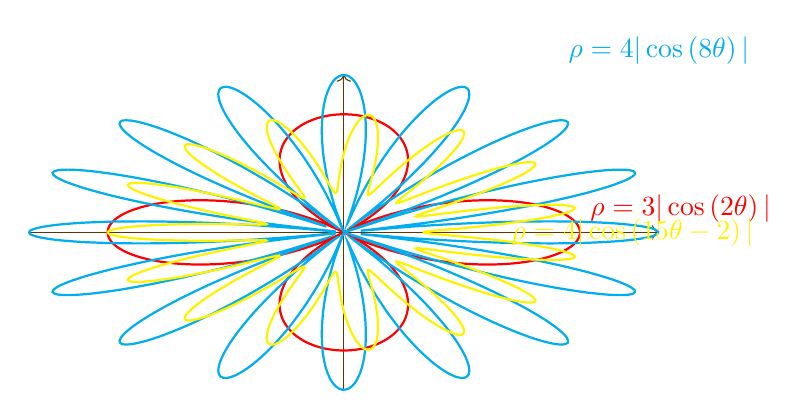
\begin{tikzpicture}[yscale=0.5]
          \draw[->,Orange](-4,0)--(4,0);
          \draw[->,Orange](0,-4)--(0,4);
          \draw[color=red, thick, domain=0:360,smooth,samples=300, variable=\t]plot ({\t}:{3*abs(cos(2*\t))}) node[above right]{\(\rho=3|\cos\left(2\theta\right)|\)};
          \draw[color=cyan, thick, domain=0:360,smooth,samples=300, variable=\t]plot ({\t}:{4*abs((cos(8*\t))}) node[above=2cm]{\(\rho=4|\cos\left(8\theta\right)|\)};
          \draw[color=yellow, thick, domain=0:360,smooth,samples=300, variable=\t]plot ({\t}:{abs((cos(15*(\t)))-2}) node[right=1cm]{\(\rho=4|\cos\left(15\theta-2\right)|\)};
    \end{tikzpicture}
  \end{lstlisting}
  \vspace{2pt}
  \begin{tikzpicture}[scale=0.6]
     \draw[draw=Blue,dashed,fill=cyan!15!white](-8,-8) rectangle (20,8);
     \node[scale=1] at (0,0) {
       \begin{tikzpicture}
   \draw[color=red, thick, domain=0:360,smooth,samples=300, variable=\t]
            plot ({\t}:{3*abs((cos(2*\t))}) node[above right]{\(\rho=3|\cos\left(2\theta\right)|\)};
    \draw[color=cyan, thick, domain=0:360,smooth,samples=300, variable=\t]
            plot ({\t}:{4*abs((cos(8*\t))}) node[above=2cm]{\(\rho=4|\cos\left(8\theta\right)|\)};
    \end{tikzpicture}
     };

\node[scale=1] at (13,0) {
       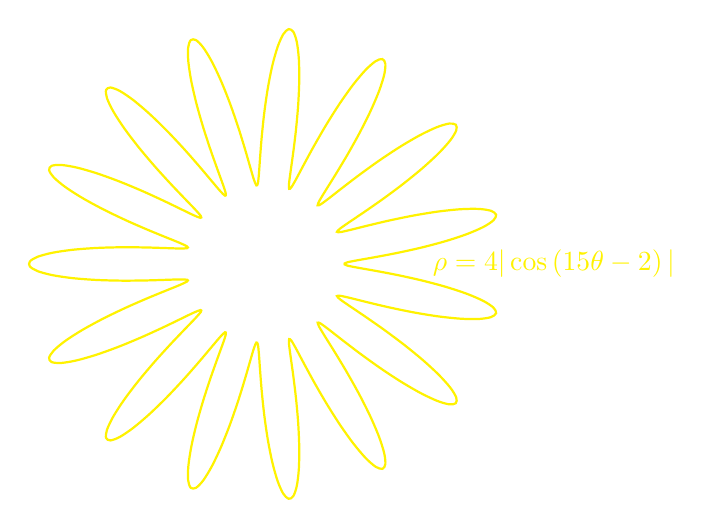
\begin{tikzpicture}
   \draw[color=yellow, thick, domain=0:360,smooth,samples=300, variable=\t]
            plot ({\t}:{abs((cos(15*(\t)))-2}) node[right=1cm]{\(\rho=4|\cos\left(15\theta-2\right)|\)};
    \end{tikzpicture}
};

   \end{tikzpicture}
\thispagestyle{empty}
\begin{tikzpicture}[scale=0.6]
     \draw[draw=Blue,dashed,fill=cyan!15!white](-8,-8) rectangle (20,8);
     \node[scale=1] at (-3,0) {
       \begin{tikzpicture}
    \draw[color=cyan, thick, domain=0:360,smooth,samples=300, fill=pink,variable=\t]
            plot ({\t}:{3*abs((sin(15*\t))});
    \end{tikzpicture}
     };

\node[scale=1] at (11,0) {
       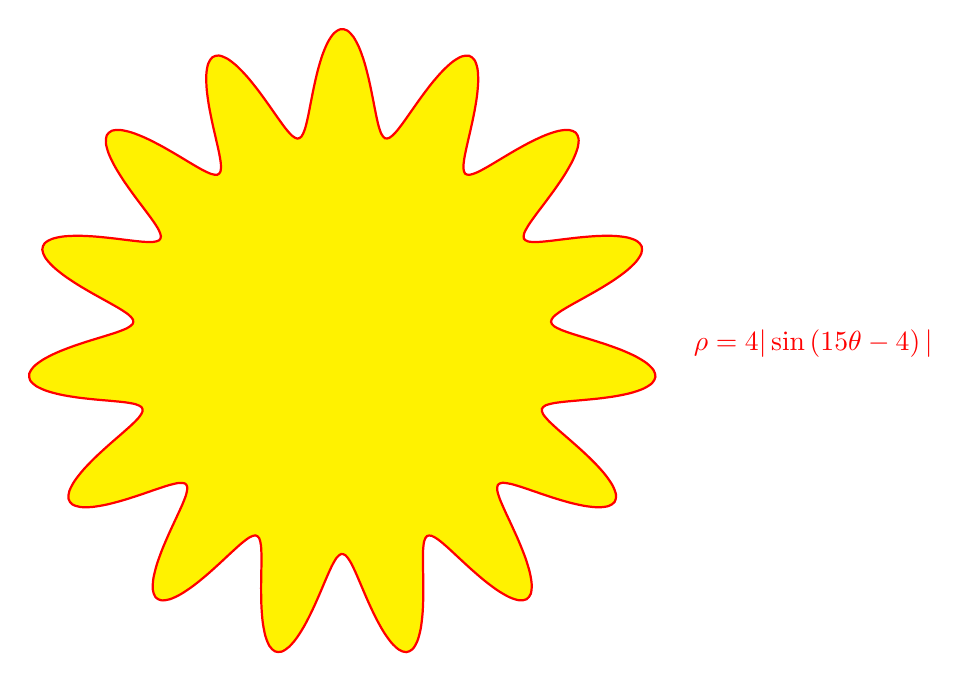
\begin{tikzpicture}
   \draw[color=red, thick, domain=0:360,smooth,samples=300, fill=yellow,variable=\t]
            plot ({\t}:{(2/3)*abs((sin(15*(\t)))-5}) node[right=1cm]{\(\rho=4|\sin\left(15\theta-4\right)|\)};
    \end{tikzpicture}
};

   \end{tikzpicture}
\thispagestyle{empty}



\clearpage
\section{TikZ/PGFplots 绘制平面几何}
 \subsection{平面的绘制}
\thispagestyle{empty}
 \vspace{3pt}
\begin{minipage}[c]{0.51\textwidth}
  \centering
  \begin{lstlisting}[gobble=8]
         \begin{tikzpicture}[scale=0.5]
          \draw[->,Orange](-1,0)--(5,0);\draw[->,Orange](0,-1)--(0,4);
          \tkzInit[ymin=-1,ymax=6,xmin=-1,xmax=10]\tkzClip[space=.5]
         \tkzDefPoint(0,0){O}\tkzDefPoint(1,0){I}\tkzDefPoint(10,0){A}
         \tkzDefMidPoint(O,A) \tkzGetPoint{M}
         \tkzDefPointWith[orthogonal](I,M)
         \tkzGetPoint{H}\tkzInterLC(I,H)(M,A)\tkzGetSecondPoint{B}
          \tkzDrawSegment(O,A)\tkzDrawSegment[style=dashed](I,H)
          \tkzDrawPoints(O,I,A,B,M)\tkzDrawArc(M,A)(O)
          \tkzMarkRightAngle(A,I,B)
          \tkzLabelSegment[right=4pt](I,B){$\sqrt{a}$}
          \tkzLabelSegment[below](O,I){$1$}
          \tkzLabelSegment[below](I,M){$a/2$}
          \tkzLabelSegment[below](M,A){$a/2$}
          \tkzLabelPoints(I,M,B,A)
          \tkzLabelPoint[below left](O){$O$}
          \end{tikzpicture}
  \end{lstlisting}
  \vspace{2pt}
\end{minipage}
\hfil
\begin{minipage}[c]{0.45\textwidth}
  \centering
  \vspace{3pt}
  \begin{tikzpicture}[scale=0.6]
     \draw[Orange,dashed](-6.5,-4)--(-6.5,4);
     \draw[draw=Blue,dashed,fill=cyan!15!white](-6,-4) rectangle (6,4);
     \node[scale=1] at (0,0) {
       \begin{tikzpicture}[scale=0.5]
         \draw[->,Orange](-1,0)--(5,0);
   \draw[->,Orange](0,-1)--(0,4);
    \tkzInit[ymin=-1,ymax=6,xmin=-1,xmax=10]
    \tkzClip[space=.5] \tkzDefPoint(0,0){O}
    \tkzDefPoint(1,0){I} \tkzDefPoint(10,0){A}
    \tkzDefMidPoint(O,A) \tkzGetPoint{M}
    \tkzDefPointWith[orthogonal](I,M)
    \tkzGetPoint{H}
    \tkzInterLC(I,H)(M,A)
    \tkzGetSecondPoint{B} \tkzDrawSegment[thick,draw=blue](O,A)
    \tkzDrawSegment[style=dashed,draw=cyan](I,H)
    \tkzDrawPoints(O,I,A,B,M)\tkzDrawArc[thick,draw=blue](M,A)(O)
    \tkzMarkRightAngle(A,I,B)
    \tkzLabelSegment[right=4pt](I,B){$\sqrt{a}$}
    \tkzLabelSegment[below](O,I){$1$}
    \tkzLabelSegment[below](I,M){$a/2$}
    \tkzLabelSegment[below](M,A){$a/2$}
    \tkzLabelPoints(I,M,B,A)
    \tkzLabelPoint[below left](O){$O$}
    \end{tikzpicture}
     };

   \end{tikzpicture}
\vspace{2pt}
\end{minipage} 

\vspace{3pt}
\begin{minipage}[c]{0.51\textwidth}
  \centering
  \begin{lstlisting}[gobble=8]
         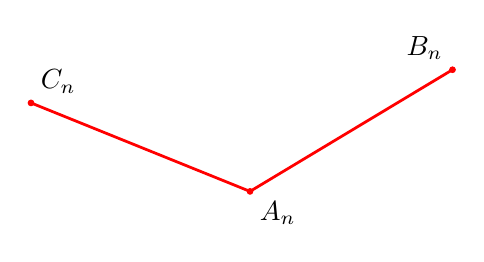
\begin{tikzpicture}
         \tkzDefPoint[label=-60:$A_n$](2,3){A}
         \tkzDefPoint[shift={(2,3)},
         label=above left:$B_n$](31:3){B}
         \tkzDefPoint[shift={(2,3)},%
         label=above right:$C_n$](158:3){C}
         \tkzDrawSegments[color=red,%
         line width=1pt](A,B A,C)
         \tkzDrawPoints[color=red](A,B,C)
         \end{tikzpicture}
  \end{lstlisting}
  \vspace{2pt}
\end{minipage}
\hfil
\begin{minipage}[c]{0.45\textwidth}
  \centering
  \vspace{3pt}
  \begin{tikzpicture}[scale=0.6]
     \draw[Orange,dashed](-6.5,-4)--(-6.5,4);
     \draw[draw=Blue,dashed,fill=cyan!15!white](-6,-4) rectangle (6,4);
     \node[scale=1] at (-2,-2) {
       \begin{tikzpicture}
\tkzDefPoint[label=-60:$A_n$](2,3){A}
\tkzDefPoint[shift={(2,3)},%
label=above left:$B_n$](31:3){B}
\tkzDefPoint[shift={(2,3)},%
label=above right:$C_n$](158:3){C}
\tkzDrawSegments[color=red,%
line width=1pt](A,B A,C)
\tkzDrawPoints[color=red](A,B,C)
\end{tikzpicture}
     };

   \end{tikzpicture}
\vspace{2pt}
\end{minipage} 


\vspace{3pt}
\begin{minipage}[c]{0.51\textwidth}
  \centering
  \begin{lstlisting}[gobble=8]
         \begin{tikzpicture}[scale=.5]\coordinate(A)at(2,3);
        \coordinate(B)at(5,-1);\tkzDefPoint[label=below:$\mathcal{C}$,
         shift={(2,3)}](-30:5.5){E}\draw(E)circle(2pt);
         \begin{scope}[shift=(A)]\tkzDefPoint(30:5){C}
         \end{scope}
         \tkzCalcLength[cm](A,B)\tkzGetLength{rAB}
         \tkzDrawCircle[R,dashed,draw=red](A,\rAB cm)
         \tkzDrawCircle(B,A)\tkzInterCC(A,B)(B,A)\tkzGetPoints{F}{G}
         \tkzLabelPoints(F,G)\tkzDrawPoints(F,G)\tkzDrawSegment(A,B)
         \tkzDrawPoints(A,B,C)\tkzLabelPoints(B,C)\tkzLabelPoints[above](A)
         \end{tikzpicture}
  \end{lstlisting}
  \vspace{2pt}
\end{minipage}
\hfil
\begin{minipage}[c]{0.45\textwidth}
  \centering
  \vspace{3pt}
  \begin{tikzpicture}[scale=0.6]
     %\draw[Orange,dashed](-6.5,-4)--(-6.5,4);
%     \draw[draw=Blue,dashed,fill=cyan!15!white](-6,-4) rectangle (6,4);
     \node[scale=1] at (-2,-2) {
       \begin{tikzpicture}[scale=0.5]
\coordinate(A)at(2,3);
\coordinate(B)at(5,-1);
\tkzDefPoint[label=below:$\mathcal{C}$,
shift={(2,3)}](-30:5.5){E}
\draw(E)circle(2pt);
\begin{scope}[shift=(A)]
\tkzDefPoint(30:5){C}
\end{scope}
\tkzCalcLength[cm](A,B)
\tkzGetLength{rAB}
\tkzDrawCircle[R,dashed,draw=red](A,\rAB
cm)
\tkzDrawCircle(B,A)
\tkzInterCC(A,B)(B,A)
\tkzGetPoints{F}{G}
\tkzLabelPoints(F,G)
\tkzDrawPoints(F,G)
\tkzDrawSegment(A,B)
\tkzDrawPoints(A,B,C)
\tkzLabelPoints(B,C)
\tkzLabelPoints[above](A)
\end{tikzpicture}
     };

   \end{tikzpicture}
\vspace{2pt}
\end{minipage}


\vspace{3pt}
\begin{minipage}[c]{0.51\textwidth}
  \centering
  \begin{lstlisting}[gobble=8]
         \begin{tikzpicture}[scale=.75]\tkzDefPoint(0,0){A}
         \tkzGetRandPointOn[circle= center A radius 4cm]{B}
         \tkzDrawPoints(A,B)
         \tkzDefPointBy[rotation= center A angle 180](B)
         \tkzGetPoint{C}\tkzInterCC[R](A,4 cm)(B,4 cm)
         \tkzGetPoints{I}{I’}\tkzInterCC[R](A,4 cm)(I,4 cm)
         \tkzGetPoints{J}{B}\tkzInterCC(B,A)(C,B)
         \tkzGetPoints{D}{E}\tkzInterCC(D,B)(E,B)
         \tkzGetPoints{M}{M’}\tikzset{arc/.style
         ={color=brown,style=dashed,delta=10}}
         \tkzDrawArc[arc](C,D)(E)\tkzDrawArc[arc,color=cyan](B,E)(D)
         \tkzDrawCircle[color=blue,line width=.2pt](A,B)
         \tkzDrawArc[arc](D,B)(M)\tkzDrawArc[arc](E,M)(B)
         \tkzCompasss[color=red,style=solid](B,II,J J,C)
         \tkzDrawPoints(B,C,D,E,M)\tkzLabelPoints(A,B,C,D,E,M,I,I’)
         \end{tikzpicture}
  \end{lstlisting}
  \vspace{2pt}
\end{minipage}
\hfil
\begin{minipage}[c]{0.45\textwidth}
  \centering
  \vspace{3pt}
  \begin{tikzpicture}[scale=0.6]
     %\draw[Orange,dashed](-6.5,-4)--(-6.5,4);
%     \draw[draw=Blue,dashed,fill=cyan!15!white](-6,-4) rectangle (6,4);
     \node[scale=1] at (-2,-2) {
       \begin{tikzpicture}[scale=.75]
\tkzDefPoint(0,0){A}
\tkzGetRandPointOn[circle= center A
radius 4cm]{B}
\tkzDrawPoints(A,B)
\tkzDefPointBy[rotation= center A
angle 180](B)
\tkzGetPoint{C}
\tkzInterCC[R](A,4 cm)(B,4 cm)
\tkzGetPoints{I}{I’}
\tkzInterCC[R](A,4 cm)(I,4 cm)
\tkzGetPoints{J}{B}
\tkzInterCC(B,A)(C,B)
\tkzGetPoints{D}{E}
\tkzInterCC(D,B)(E,B)
\tkzGetPoints{M}{M’}
\tikzset{arc/.style
={color=brown,style=dashed,delta=10}}
\tkzDrawArc[arc](C,D)(E)
\tkzDrawArc[arc,color=cyan](B,E)(D)
\tkzDrawCircle[color=blue,line
width=.2pt](A,B)
\tkzDrawArc[arc](D,B)(M)
\tkzDrawArc[arc](E,M)(B)
\tkzCompasss[color=red,style=solid](B,I
I,J J,C)
\tkzDrawPoints(B,C,D,E,M)
\tkzLabelPoints(A,B,C,D,E,M,I,I’)
\end{tikzpicture}
     };

   \end{tikzpicture}
\vspace{2pt}
\end{minipage}


\vspace{3pt}
\begin{minipage}[c]{0.51\textwidth}
  \centering
  \begin{lstlisting}[gobble=8]
         \begin{tikzpicture}[scale=.8]
         \tkzDefPoint(0,0){A}
         \tkzDefPoint(5,0){B}
         \tkzDrawCircle[R,dashed](A,4 cm)
         \tkzDrawCircle[R,dashed](B,3 cm)
         \tkzInterCC[R](A,4 cm)(B,3 cm)
         \tkzGetPoints{C}{D}
         \tkzDrawPolygon(A,B,C)
         \tkzCompasss(A,C B,C)
         \tkzLabelSegment[below](A,B){$5$ cm}
         \tkzLabelSegment[above left](A,C){$4$ cm}
         \tkzLabelSegment[above
         right](B,C){$3$ cm}
         \tkzDrawPoints[color=red](C)
         \tkzDrawPoints[color=blue](A,B)
         \end{tikzpicture}
  \end{lstlisting}
  \vspace{2pt}
\end{minipage}
\hfil
\begin{minipage}[c]{0.45\textwidth}
  \centering
  \vspace{3pt}
  \begin{tikzpicture}[scale=0.5]
     %\draw[Orange,dashed](-6.5,-4)--(-6.5,4);
%     \draw[draw=Blue,dashed,fill=cyan!15!white](-6,-4) rectangle (6,4);
     \node[scale=1] at (-2,-2) {
       \begin{tikzpicture}[scale=.7]
\tkzDefPoint(0,0){A}
\tkzDefPoint(5,0){B}
\tkzDrawCircle[R,dashed,draw=cyan](A,4 cm)
\tkzDrawCircle[R,dashed,draw=blue](B,3 cm)
\tkzInterCC[R](A,4 cm)(B,3 cm)
\tkzGetPoints{C}{D}
\tkzDrawPolygon(A,B,C)
\tkzCompasss(A,C B,C)
\tkzLabelSegment[below](A,B){$5$ cm}
\tkzLabelSegment[above left](A,C){$4$
cm}
\tkzLabelSegment[above
right](B,C){$3$ cm}
\tkzDrawPoints[color=red](C)
\tkzDrawPoints[color=blue](A,B)
\end{tikzpicture}
     };

   \end{tikzpicture}
\vspace{2pt}
\end{minipage}

\thispagestyle{empty}
\vspace{3pt}
\begin{minipage}[c]{0.51\textwidth}
  \centering
  \begin{lstlisting}[gobble=8]
         \begin{tikzpicture}[scale=1.25]
         \tkzInit[xmin= 0,xmax=8 ,ymin=0 ,ymax=7 ] \tkzClip[space=.5]
         \tkzDefPoint(0,0){C}\tkzDefPoint(7,0){B}
         \tkzDefPoint(5,6){A}\tkzDrawPolygon(A,B,C)
         \tkzDefMidPoint(C,B)\tkzGetPoint{I}
         \tkzDrawArc(I,B)(C)\tkzInterLC(A,C)(I,B)
         \tkzGetSecondPoint{B’}\tkzInterLC(A,B)(I,B)
         \tkzGetFirstPoint{C’}\tkzInterLL(B,B’)(C,C’)
         \tkzGetPoint{H}\tkzInterLL(A,H)(C,B)\tkzGetPoint{A’}
         \tkzDrawCircle[circum,color=red](A,B’,C’)
         \tkzDrawSegments[color=orange](B,B’ C,C’ A,A’)
         \tkzMarkRightAngles(C,B’,B B,C’,C C,A’,A)
         \tkzDrawPoints(A,B,C,A’,B’,C’,H)
         \tkzLabelPoints(A,B,C,A’,B’,C’,H)
         \end{tikzpicture}
  \end{lstlisting}
  \vspace{2pt}
\end{minipage}
\hfil
\begin{minipage}[c]{0.45\textwidth}
  \centering
  \vspace{3pt}
  \begin{tikzpicture}[scale=0.5]
     %\draw[Orange,dashed](-6.5,-4)--(-6.5,4);
%     \draw[draw=Blue,dashed,fill=cyan!15!white](-6,-4) rectangle (6,4);
     \node[scale=1] at (-2,-2) {
       \begin{tikzpicture}[scale=1]
\tkzInit[xmin= 0,xmax=8 ,ymin=0 ,ymax=7 ] \tkzClip[space=.5]
\tkzDefPoint(0,0){C}
\tkzDefPoint(7,0){B}
\tkzDefPoint(5,6){A}
\tkzDrawPolygon(A,B,C)
\tkzDefMidPoint(C,B)
\tkzGetPoint{I}
\tkzDrawArc(I,B)(C)
\tkzInterLC(A,C)(I,B)
\tkzGetSecondPoint{B’}
\tkzInterLC(A,B)(I,B)
\tkzGetFirstPoint{C’}
\tkzInterLL(B,B’)(C,C’)
\tkzGetPoint{H}
\tkzInterLL(A,H)(C,B)
\tkzGetPoint{A’}
\tkzDrawCircle[circum,color=cyan](A,B’,C’)
\tkzDrawSegments[color=orange,dashed](B,B’ C,C’ A,A’)
\tkzMarkRightAngles(C,B’,B B,C’,C C,A’,A)
\tkzDrawPoints(A,B,C,A’,B’,C’,H)
\tkzLabelPoints(A,B,C,A’,B’,C’,H)
\end{tikzpicture}
     };

   \end{tikzpicture}
\vspace{2pt}
\end{minipage}


\vspace{5pt}
\begin{minipage}[c]{0.51\textwidth}
  \centering
  \begin{lstlisting}[gobble=8]
         \begin{tikzpicture}[scale=0.7]
         \tkzInit[xmin=-3,xmax=6,ymin=-1,ymax=6]
         \tkzDrawX[noticks]\tkzDrawY[noticks]
         \tkzDefPoint(0,0){O}\tkzDefPoint(4,2){A}
         \tkzDefPoint(-2,6){B}
         \tkzPointShowCoord[xlabel=$x$,ylabel=$y$](A)
         %%显示点的坐标
         \tkzPointShowCoord[xlabel=$x’$,ylabel=$y’$,%
         ystyle={right=2pt}](B)\tkzDrawVectors(O,A O,B)
         \tkzLabelSegment[above=3pt](O,A){$\vec{u}$}
         \tkzLabelSegment[above=3pt](O,B){$\vec{v}$}
         \tkzMarkAngle[fill=yellow,size=1.8cm,%opacity=.5](A,O,B)
         \tkzFillPolygon[red!30,opacity=0.25](A,B,O)
         \tkzLabelAngle[pos =
         1.5](A,O,B){$\alpha$}
         \end{tikzpicture}
  \end{lstlisting}
  \vspace{2pt}
\end{minipage}
\hfil
\begin{minipage}[c]{0.45\textwidth}
  \centering
  \vspace{3pt}
  \begin{tikzpicture}[scale=0.5]
     %\draw[Orange,dashed](-6.5,-4)--(-6.5,4);
%     \draw[draw=Blue,dashed,fill=cyan!15!white](-6,-4) rectangle (6,4);
     \node[scale=1] at (-2,-2) {
       \begin{tikzpicture}[scale=0.7]
\tkzInit[xmin=-3,xmax=6,ymin=-1,ymax=6]
\tkzDrawX[noticks]
\tkzDrawY[noticks]
\tkzDefPoint(0,0){O}
\tkzDefPoint(4,2){A}
\tkzDefPoint(-2,6){B}
\tkzPointShowCoord[xlabel=$x$,ylabel=$y$](A)
%%显示点的坐标
\tkzPointShowCoord[xlabel=$x’$,ylabel=$y’$,%
ystyle={right=2pt}](B)
\tkzDrawVectors(O,A O,B)
\tkzLabelSegment[above=3pt](O,A){$\vec{u}$}
\tkzLabelSegment[above=3pt](O,B){$\vec{v}$}
\tkzMarkAngle[fill=
yellow,size=1.8cm,%
opacity=.5](A,O,B)
\tkzFillPolygon[red!30,opacity=0.25](A,B,O)
\tkzLabelAngle[pos =
1.5](A,O,B){$\alpha$}
\end{tikzpicture}
     };

   \end{tikzpicture}
\vspace{2pt}
\end{minipage}

\vspace{3pt}
\begin{minipage}[c]{0.51\textwidth}
  \centering
  \begin{lstlisting}[gobble=8]
         \begin{tikzpicture}[scale=0.6]
         \tkzInit[xmin=-4.1,xmax=5.2,ymin=-4.1,ymax=8]
         \tkzClip[space=.5]
         \tkzDefPoint(100:8){A}\tkzDefPoint(50:8){B}
         \tkzDefPoint(0,0){C}
         \tkzDefPoint(0,4){R}
         \tkzDrawCircle(C,R)
         \tkzTangent[from = A](C,R)
         \tkzGetPoints{D}{E}
         \tkzTangent[from = B](C,R)
         \tkzGetPoints{F}{G}
         \tkzDrawSector[fill=blue!80!black,opacity=0.5](A,D)(E)
         \tkzFillSector[color=red!80!black,opacity=0.5](B,F)(G)
         \tkzInterCC(A,D)(B,F)
         \tkzGetSecondPoint{I}
         \tkzDrawPoint[color=black](I)
         \end{tikzpicture}
  \end{lstlisting}
  \vspace{2pt}
\end{minipage}
\hfil
\begin{minipage}[c]{0.45\textwidth}
  \centering
  \vspace{3pt}
  \begin{tikzpicture}[scale=0.5]
     %\draw[Orange,dashed](-6.5,-4)--(-6.5,4);
%     \draw[draw=Blue,dashed,fill=cyan!15!white](-6,-4) rectangle (6,4);
     \node[scale=1] at (-2,-2) {
       \begin{tikzpicture}[scale=0.6]
\tkzInit[xmin=-4.1,xmax=5.2,ymin=-4.1,ymax=8]
\tkzClip[space=.5]
\tkzDefPoint(100:8){A}\tkzDefPoint(50:8){B}
\tkzDefPoint(0,0){C}
\tkzDefPoint(0,4){R}
\tkzDrawCircle[draw=blue,thick,dashed](C,R)
\tkzTangent[from = A](C,R)
\tkzGetPoints{D}{E}
\tkzTangent[from = B](C,R)
\tkzGetPoints{F}{G}
\tkzDrawSector[fill=blue!80!black,opacity=0.5](A,D)(E)
\tkzFillSector[color=red!80!black,opacity=0.5](B,F)(G)
\tkzInterCC(A,D)(B,F)
\tkzGetSecondPoint{I}
\tkzDrawPoint[color=black](I)
\end{tikzpicture}
     };

   \end{tikzpicture}
\vspace{2pt}
\end{minipage}

\thispagestyle{empty}
\vspace{3pt}
\begin{minipage}[c]{0.51\textwidth}
  \centering
  \begin{lstlisting}[gobble=8]
         \begin{tikzpicture}
         \tkzInit[xmin=-1,ymin=-1,xmax=8,ymax=6]
         \tkzClip
         \tkzDefPoint(5,3.5){A}
         \tkzDefPoint(0,0){B}
         \tkzDefPoint(7,0){C}
         \tkzDefCircle[euler](A,B,C)
         \tkzGetPoint{E}
         \tkzGetLength{rEuler}
         \tkzDrawPoints(A,B,C,E)
         \tkzDrawCircle[R,draw=cyan,thick]
         (E,\rEuler pt)
         \tkzDrawPolygon(A,B,C)
         \tkzLabelPoints[below](B,C)
         \tkzLabelPoints[left](A,E)
         \end{tikzpicture}
  \end{lstlisting}
  \vspace{2pt}
\end{minipage}
\hfil
\begin{minipage}[c]{0.45\textwidth}
  \centering
  \vspace{3pt}
  \begin{tikzpicture}[scale=0.7]
     \draw[Orange,dashed](-6.5,-4)--(-6.5,4);
     \draw[draw=Blue,dashed,fill=cyan!15!white](-6,-4) rectangle (6,4);
     \node[scale=1] at (0,0) {
       \begin{tikzpicture}
\tkzInit[xmin=-1,ymin=-1,xmax=8,ymax=6]
\tkzClip
\tkzDefPoint(5,3.5){A}
\tkzDefPoint(0,0){B}
\tkzDefPoint(7,0){C}
\tkzDefCircle[euler](A,B,C)
\tkzGetPoint{E}
\tkzGetLength{rEuler}
\tkzDrawPoints(A,B,C,E)
\tkzDrawCircle[R,draw=cyan,thick](E,\rEuler pt)
\tkzDrawPolygon(A,B,C)
\tkzLabelPoints[below](B,C)
\tkzLabelPoints[left](A,E)
\end{tikzpicture}
     };

   \end{tikzpicture}
\vspace{2pt}
\end{minipage}


\clearpage
\thispagestyle{empty}
\vspace{3pt}
\begin{minipage}[c]{0.51\textwidth}
  \centering
  \begin{lstlisting}[gobble=8]
         \begin{tikzpicture}[scale=0.45]
         \tkzInit[xmin=-9,ymin=-6,xmax=9,ymax=6]
         \tkzClip
         \tkzDefPoint(0,0){O}
         \tkzDefPoint(132:4){A}
         \tkzDefPoint(5,0){B}
         \foreach \ang in {5,10,...,360}{%
         \tkzDefPoint(\ang:5){M}
         \tkzDefLine[mediator](A,M)
         \tkzDrawLine[color=blue,add= 4 and
         4](tkzFirstPointResult,
         tkzSecondPointResult)}
         \tkzDrawPoints(O,A,B)
         \tkzLabelPoints(O,A,B)
         \end{tikzpicture}
  \end{lstlisting}
  \vspace{2pt}
\end{minipage}
\hfil
\begin{minipage}[c]{0.45\textwidth}
  \centering
  \vspace{3pt}
  \begin{tikzpicture}[scale=0.7]
     \draw[Orange,dashed](-6.5,-4)--(-6.5,4);
     \draw[draw=Blue,dashed,fill=cyan!15!white](-6,-4) rectangle (6,4);
     \node[scale=1] at (0,0) {
       \begin{tikzpicture}[scale=0.45]
\tkzInit[xmin=-9,ymin=-6,xmax=9,ymax=6]
\tkzClip
\tkzDefPoint(0,0){O}
\tkzDefPoint(132:4){A}
\tkzDefPoint(5,0){B}
\foreach \ang in {5,10,...,360}{%
\tkzDefPoint(\ang:5){M}
\tkzDefLine[mediator](A,M)
\tkzDrawLine[color=green,add= 4 and
4](tkzFirstPointResult,tkzSecondPointResult)}
\tkzDrawPoints(O,A,B)\tkzLabelPoints(O,A,B)
\end{tikzpicture}
     };

   \end{tikzpicture}
\vspace{2pt}
\end{minipage}



\vspace{3pt}
\begin{minipage}[c]{0.51\textwidth}
  \centering
  \begin{lstlisting}[gobble=8]
         \begin{tikzpicture}[scale=0.45]
         \tkzInit[xmin=-9,ymin=-6,xmax=9,ymax=6]
         \tkzClip
         \tkzDefPoint(0,0){O}
         \tkzDefPoint(132:4){A}
         \tkzDefPoint(5,0){B}
         \foreach \ang in {5,10,...,360}{%
         \tkzDefPoint(\ang:5){M}
         \tkzDefLine[mediator](A,M)
         \tkzDrawLine[color=blue,add= 4 and
         4](tkzFirstPointResult,
         tkzSecondPointResult)}
         \tkzDrawPoints(O,A,B)
         \tkzLabelPoints(O,A,B)
         \end{tikzpicture}
  \end{lstlisting}
  \vspace{2pt}
\end{minipage}
\hfil
\begin{minipage}[c]{0.45\textwidth}
  \centering
  \vspace{3pt}
  \begin{tikzpicture}[scale=0.7]
     \draw[Orange,dashed](-6.5,-4)--(-6.5,4);
     \draw[draw=Blue,dashed,fill=pink!15!white](-6,-4) rectangle (6,4);
     \node[scale=1] at (0,0) {
       \begin{tikzpicture}[scale=0.45]
\tkzInit[xmin=-9,ymin=-6,xmax=9,ymax=6]
\tkzClip
\tkzDefPoint(0,0){O}
\tkzDefPoint(132:5){A}
\tkzDefPoint(4,0){B}
\foreach \ang in {5,10,...,360}{%
\tkzDefPoint(\ang:4){M}
\tkzDefLine[mediator](A,M)
\tkzDrawLine[color=blue,
add= 4 and 4](tkzFirstPointResult,tkzSecondPointResult)}
\tkzDrawPoints(O,A,B)\tkzLabelPoints(O,A,B)
\end{tikzpicture}
     };

   \end{tikzpicture}
\vspace{2pt}
\end{minipage}

\vspace{3pt}
\begin{minipage}[c]{0.51\textwidth}
  \centering
  \begin{lstlisting}[gobble=8]
         \begin{tikzpicture}[scale=0.7]
         \draw[Orange,dashed](-6.5,-4)--(-6.5,4);
         \draw[draw=Blue,dashed,
         fill=pink!15!white](-6,-4) rectangle (6,4);
         \node[scale=1] at (0,0) {
         \begin{tikzpicture}[scale=0.8]
         \tkzDefPoint(0,0){O}
         \tkzDefPoint(2,0){A}
         \foreach \ang in {5,10,...,360}{
         \tkzDefPoint(\ang:2){M}
         \tkzDrawCircle[draw=cyan](M,A)
         }
         \end{tikzpicture}
         };
         \end{tikzpicture}
  \end{lstlisting}
  \vspace{2pt}
\end{minipage}
\hfil
\begin{minipage}[c]{0.45\textwidth}
  \centering
  \vspace{3pt}
  \begin{tikzpicture}[scale=0.7]
     \draw[Orange,dashed](-6.5,-4)--(-6.5,4);
     \draw[draw=Blue,dashed,fill=pink!15!white](-6,-4) rectangle (6,4);
     \node[scale=1,rotate=90] at (0,0) {
       \begin{tikzpicture}[scale=0.6]
\tkzDefPoint(0,0){O}
\tkzDefPoint(2,0){A}
\foreach \ang in {5,10,...,360}{%
\tkzDefPoint(\ang:2){M}
\tkzDrawCircle[draw=cyan](M,A)
}
\end{tikzpicture}
     };

   \end{tikzpicture}
\vspace{2pt}
\end{minipage}

\begin{lstlisting}[gobble=8]
         \begin{tikzpicture}[scale=.333]\tkzInit[xmin=-10,xmax=10,ymin=-10,ymax=10]
         \tkzDefPoint(0 , 0){O}\tkzDefPoint(9,0){A}
         \tkzDefPoint(-9, 0){C}\tkzDefPoint(0,9){B}
         \tkzDefPoint(0 ,-9){D}\tkzClipCircle(O,A)
         \foreach \pti in {1,2,...,8}{
         \tkzDefPoint(10*\pti:9){P\pti}\tkzDefPoint(90:\pti){MP\pti}
         \tkzDefPoint(0: \pti){NP\pti}\tkzDefLine[mediator](MP\pti,P\pti)
         \tkzInterLL(B,D)(tkzFirstPointResult,tkzSecondPointResult)
         \tkzDrawCircle[color=cyan](tkzPointResult,P\pti)}
         \foreach \pti in {-1,-2,...,-8}{\tkzDefPoint(10*\pti:9){P\pti}
         \tkzDefPoint(-90:-\pti){MP\pti}\tkzDefPoint(0: -\pti){NP\pti}
         \tkzDefLine[mediator](MP\pti,P\pti)
         \tkzInterLL(B,D)(tkzFirstPointResult,tkzSecondPointResult)
         \tkzDrawCircle[color=cyan](tkzPointResult,P\pti)}
         \foreach \pti in {1,2,...,8}{\tkzDefLine[mediator](B,NP\pti)
         \tkzInterLL(A,C)(tkzFirstPointResult,tkzSecondPointResult)
         \tkzDrawCircle[color=cyan](tkzPointResult,NP\pti)}
         \foreach \pti in {1,2,...,8}{\tkzDefPoint(0: -\pti){NP\pti}
         \tkzDefLine[mediator](B,NP\pti)
         \tkzInterLL(A,C)(tkzFirstPointResult,tkzSecondPointResult)
         \tkzDrawCircle[color=cyan](tkzPointResult,NP\pti)}
         \tkzDrawCircle[R,color=cyan](O,9cm)\tkzDrawSegments[color=cyan](A,CB,D)
         \end{tikzpicture}
\end{lstlisting}

\thispagestyle{empty}
\begin{tikzpicture}[scale=.4]
\tkzInit[xmin=-10,xmax=10,ymin=-10,ymax=10]
\tkzDefPoint(0 , 0){O}\tkzDefPoint(9 ,
0){A}
\tkzDefPoint(-9, 0){C}\tkzDefPoint(0 ,
9){B}
\tkzDefPoint(0 ,-9){D}
\tkzClipCircle(O,A)
\foreach \pti in {1,2,...,8}{
\tkzDefPoint(10*\pti:9){P\pti}
\tkzDefPoint(90:\pti){MP\pti}
\tkzDefPoint(0: \pti){NP\pti}
\tkzDefLine[mediator](MP\pti,P\pti)
\tkzInterLL(B,D)(tkzFirstPointResult,tkzSecondPointResult)
\tkzDrawCircle[color=cyan](tkzPointResult,P\pti)
}
\foreach \pti in {-1,-2,...,-8}{
\tkzDefPoint(10*\pti:9){P\pti}
\tkzDefPoint(-90:-\pti){MP\pti}
\tkzDefPoint(0: -\pti){NP\pti}
\tkzDefLine[mediator](MP\pti,P\pti)
\tkzInterLL(B,D)(tkzFirstPointResult,tkzSecondPointResult)
\tkzDrawCircle[color=cyan](tkzPointResult,P\pti)
}
\foreach \pti in {1,2,...,8}{
\tkzDefLine[mediator](B,NP\pti)
\tkzInterLL(A,C)(tkzFirstPointResult,tkzSecondPointResult)
\tkzDrawCircle[color=cyan](tkzPointResult,NP\pti)
}
\foreach \pti in {1,2,...,8}{
\tkzDefPoint(0: -\pti){NP\pti}
\tkzDefLine[mediator](B,NP\pti)
\tkzInterLL(A,C)(tkzFirstPointResult,tkzSecondPointResult)
\tkzDrawCircle[color=cyan](tkzPointResult,NP\pti)
}
\tkzDrawCircle[R,color=cyan](O,9
cm)
\tkzDrawSegments[color=cyan](A,C
B,D)
\end{tikzpicture}
\hfill
\begin{tikzpicture}[scale=1]
     \foreach \i in {0,0.01,...,2}
 \draw[draw=orange,rotate=-124]($(0,0) !1! \i*180:(3,2)$)--($(0,0) !1! \i*7720:(3,2)$);
    \end{tikzpicture}

\begin{lstlisting}[gobble=8]
      \begin{tikzpicture}[scale=1]
      \foreach \i in {0,0.01,...,2}\draw[draw=green,rotate=-124]($(0,0) !1! \i*180:(3,2)$)--($(1,1) !1! \i*1620:(3,3)$);
      \end{tikzpicture}
\end{lstlisting}
\begin{tikzpicture}[scale=1]
     \foreach \i in {0,0.01,...,2}
 \draw[draw=green,rotate=-124]($(0,0) !1! \i*180:(3,2)$)--($(1,1) !1! \i*1620:(3,3)$);
    \end{tikzpicture}
    \hfill
\begin{tikzpicture}[scale=1]
     \foreach \i in {0,0.01,...,2}
 \draw[draw=violet,rotate=-124]($(0,0) !1! \i*180:(3,2)$)--($(2,2) !1! \i*7200:(3,3)$);
    \end{tikzpicture}


\begin{lstlisting}[gobble=8]
      \begin{tikzpicture}[scale=1]
      \foreach \i in {0,0.01,...,2}\draw[draw=green,rotate=-124]($(0,0) !1! \i*180:(3,2)$)--($(1,1) !1! \i*1620:(3,3)$);
      \end{tikzpicture}
\end{lstlisting}

\clearpage
\section{TikZ/PGFplots + Animate 绘制动画}

\begin{lstlisting}[gobble=8]
           \documentclass{beamer}
           \usepackage{tikz, tkz-euclide}
           \usepackage{animate}
           \usetikzlibrary{math, calc}
           \begin{document}
           \begin{animateinline}[poster=31, controls={play,step,stop}]{24}
            \multiframe{361}{rtheta=0+1}
            {\begin{tikzpicture}[scale=1]
                    \path[use as bounding box] (-3.5,-2) rectangle (7.2,2;
                    \draw[rounded corners] (-3.5,-2) rectangle (7.2,2);
                    \tikzmath{function fCosseno(\x){return cos(\x);};
                        function degreeToRad(\d){ return {pi}*\d/180;};}
                    \draw[->,>=latex,thick] (-0.3,0) -- (7,0)node[below]{\(x\)};
                    \draw[->,>=latex,thick] (0,-1.5) -- (0,1.5)node[left]{\(y\)};
                    \draw[ultra thick, red, samples=50, domain=0:{2*pi}] plot (\x, {cos(\x r)});
                    \node at (0,0) [below left]{\(O\)};
                    \node at ({pi/2},0) [below]{\(\frac{\pi}{2}\)};
                    \node at ({pi},0) [below]{\(\pi\)};
                    \node at ({3*pi/2},0) [below]{\(\frac{3\pi}{2}\)};
                    \node at ({2*pi},0) [below]{\(2\pi\)};
                    \draw[thin, dashed] ({2*pi}, 0) -- ({2*pi},1);\draw (-2,0) circle (1cm);
                    \draw[->,>=latex,thick] (-3.5,0) -- (-0.5,0);
                    \draw[->,>=latex,thick] (-2,-1.5) -- (-2,1.5);
                    \coordinate (A) at (-2,0);\coordinate (B) at (-2,1);
                    \coordinate (C) at (-2,-1);\coordinate (D) at (-3,0);
                    \coordinate (E) at (-1,0);\coordinate (P) at ($(A) + (\rtheta:1)$);
                    \draw[thick] (A) -- (P);
                    \draw[thin, dashed, red] ($(D)!(P)!(E)$) -- (P) -- ($(B)!(P)!(C)$);
                    \draw[->, >=stealth] (-1.6,0) arc [start angle=0, end angle=\rtheta, radius=0.4];
                    \coordinate (Q) at ($(A) + ({fCosseno(\rtheta)},0)$);
                    \coordinate (R) at ($({-2+fCosseno(\rtheta)}, {fCosseno(\rtheta)})$);
                    \draw[ultra thick, red] (A) -- (Q) -- (R);
                    \tkzDrawArc[thin, red](Q,R)(A)
                    \draw[thin, red, dashed] (R) -- ({degreeToRad(\rtheta)}, {fCosseno(\rtheta)}) -- ({degreeToRad(\rtheta)},0);
                    \draw[fill=black] ({degreeToRad(\rtheta)}, {fCosseno(\rtheta)}) circle (1pt);
                \end{tikzpicture}}
         \end{animateinline}
        \end{document}
\end{lstlisting}

        \begin{tikzpicture}[scale=1.6]
            \path[use as bounding box] (-3.5,-2) rectangle (7.2,2);
            \draw[rounded corners,fill=cyan!20!white] (-3.5,-2) rectangle (7.2,2);

            \tikzmath{
                function fCosseno(\x){
                    return cos(\x);
                };
                function degreeToRad(\d){
                    return {pi}*\d/180;
                };
            }
            \draw[->,>=latex,thick] (-0.3,0) -- (7,0)node[below]{\(x\)};
            \draw[->,>=latex,thick] (0,-1.5) -- (0,1.5)node[left]{\(y\)};
            \draw[ultra thick, red, samples=50, domain=0:{2*pi}]
            plot (\x, {cos(\x r)});
            \node at (0,0) [below left]{\(O\)};
            \node at ({pi/2},0) [below]{\(\frac{\pi}{2}\)};
            \node at ({pi},0) [below]{\(\pi\)};
            \node at ({3*pi/2},0) [below]{\(\frac{3\pi}{2}\)};
            \node at ({2*pi},0) [below]{\(2\pi\)};
            \draw[thin, dashed] ({2*pi}, 0) -- ({2*pi},1);
            \draw (-2,0) circle (1cm);
            \draw[->,>=latex,thick] (-3.5,0) -- (-0.5,0);
            \draw[->,>=latex,thick] (-2,-1.5) -- (-2,1.5);
            \coordinate (A) at (-2,0);
            \coordinate (B) at (-2,1);
            \coordinate (C) at (-2,-1);
            \coordinate (D) at (-3,0);
            \coordinate (E) at (-1,0);
            \coordinate (P) at ($(A) + ( 60:1)$);
            \draw[thick] (A) -- (P);
            \draw[thin, dashed, red] ($(D)!(P)!(E)$) -- (P) -- ($(B)!(P)!(C)$);
            \draw[->, >=stealth] (-1.6,0) arc [start angle=0, end angle= 60, radius=0.4];
            \coordinate (Q) at ($(A) + ({fCosseno( 60)},0)$);
            \coordinate (R) at ($({-2+fCosseno( 60)}, {fCosseno( 60)})$);
            \draw[ultra thick, red] (A) -- (Q) -- (R);
            \tkzDrawArc[thin, red](Q,R)(A)
            \draw[thin, red, dashed] (R) -- ({degreeToRad( 60)}, {fCosseno( 60)}) -- ({degreeToRad( 60)},0);
            \draw[fill=black] ({degreeToRad( 60)}, {fCosseno( 60)}) circle (1pt);
        \end{tikzpicture}
 
\section{TikZ/PGFplots 科学绘图}
 \subsection{PGFplots 数据绘图}
 \subsection{PGFplots 函数绘图}


\end{document} 